% -*- root: ../../main.tex -*
%!TEX root = ../../main.tex
% vim:textwidth=80 fo=cqt conceallevel=0

\graphicspath{{chapters/layer_opt/figures/}}
% ----------------------- contents from here ------------------------

\chapter{Model-based Design Of Pouch Cells}\label{ch:modelbaseddesign}
\vspace*{-1em}
\startcontents[chapters]
\printcontents[chapters]{}{1}{\setcounter{tocdepth}{1}}

\bigskip

\glsunset{xeV}

%% A brief  1-2 sentences throwback to  the literature review, referring  what I
%% will say in this chapter.

\section[Introduction]{Introduction\protect\footnote{\textbf{Attribution      of
        content}  \   The  groundwork   for  converting   the  existing   computer  code
        (LIONSIMBA~v1.0$x$) into a suitable form for layer optimisation was initiated by
        this  thesis  author,  \mbox{Krishnakumar  Gopalakrishnan}.  However,  with  the
        exception of  the spectral scheme, for  which \mbox{Krishnakumar Gopalakrishnan}
        was  responsible, and  the zero-dimensional  thermal model  for which  \mbox{Ian
        Campbell} was  responsible, the advancements  inherent to the  enhanced computer
        software  (LIONSIMBA~v2.0)  were  made  in  equal  parts  by  \mbox{Krishnakumar
        Gopalakrishnan} and \mbox{Ian Campbell}. These  advancements would not have been
        possible without the contributions and support of Dr.~Davide Raimondo who served
        as an unofficial  supervisor for the work reported in  this chapter. The concept
        of layer reconfiguration for energy  and power trade-off, the layer optimisation
        framework, and the  source code by which it is  implemented were co-developed in
        equal  parts  by  \mbox{Krishnakumar Gopalakrishnan}  and  \mbox{Ian  Campbell}.
        \mbox{Krishnakumar Gopalakrishnan} was the  major contributor to the development
        of the binary search while \mbox{Ian  Campbell} was the major contributor in the
        analysis of results. \mbox{Parvathy  Chittur Subramanianprasad} was instrumental
        in  developing the  analytical expression  for  the maximum  possible number  of
layers~$n_\text{max}$.}}\label{sec:layeroptintro}
% -*- root: ../../main.tex -*
%!TEX root = ../../main.tex
% vim:textwidth=80 fo=cqt conceallevel=0


\capolettera{T}{he} issue of `range anxiety'  is a pervasive mental blockade for
potential buyers  of electric  vehicles which  in-turn hampers  their widespread
adoption. From  a consumer viewpoint,  yet another  practical issue is  the fact
that on  encountering a `low battery'  scenario in a long  distance journey, the
charging  times required  for sufficiently  replenishing the  battery to  enable
completion  of the  journey  are  prohibitively large,  to  the  point of  being
non-competitive against conventional fossil fuel powered vehicles.

Unfortunately,  the  aforementioned  scenarios  are not  unimaginable  with  the
present  state  of the  art  in  lithium  ion  batteries. Hence,  improving  the
\gls{aer} and  providing fast charging  capabilities are two near-term  goals of
manufacturers  of electric  vehicles.  Increasing the  \gls{aer} necessitates  a
battery pack with  higher energy content in it while  lowering the charging time
demands a  pack with higher  power capability.  The contrasting nature  of these
goals can  be traced  all the way  down to  the cell level  and is  presented in
\cref{sec:energypowertradeoff}. By trading  off the number of layers  in a pouch
cell  against  the content  of  active  electrode material  accommodated  within
it,  bespoke cell  designs  addressing either  the energy  demand  or the  power
demand  can  be  obtained.  In  the  absence  of  accessible  documentation  (as
either  industry white  papers or  academic literature)  on the  layer selection
methodologies employed in automotive pouch  cell designs, this author postulates
that manufacturers  iterate through  an extensive  empirical testing  process of
prototypes with  a range of  layer choices. In the  view of this  thesis author,
this  procedure is  not only  time-consuming, but  is also  likely to  result in
sub-optimal designs.  This chapter envisages a  model-based engineering solution
to more  optimal cell designs  by determining  the appropriate number  of layers
needed  to maximise  its  \emph{usable} energy  while simultaneously  satisfying
certain  power  capability constraints.  The  rest  of  the chapter  provides  a
detailed treatment of topics such  as the proposed layer optimisation framework,
its assumptions involved,  and various modifications to  standard numerical code
required to facilitate this design procedure.



\section{Energy/Power Trade-off in Pouch Cells by Layer Selection}\label{sec:energypowertradeoff}
% -*- root: ../../main.tex -*
%!TEX root = ../../main.tex
% vim:textwidth=80 fo=cqt conceallevel=0


Varying the  number of electrochemical  layers stacked  within a pouch  cell has
contrasting effects  on its energy  storage and power handling  capabilities. In
this section,  a high-level  intuitive explanation of  this phenomenon  is first
offered, before  delving into  a detailed  presentation of  this effect  and its
implications for a specific  example cell in \cref{sec:energypowertradeoffdemo}.
Interwoven into the  narrative is a set of simplifying  assumptions made by this
thesis  author, which  sets the  broader  context within  which a  computational
framework for  determining the optimum  number of  layers for a  specific target
design shall be formalised and presented in \cref{sec:layeroptframework}.

\subsection{Preliminary assumptions}\label{subsec:layeroptassumptions}

To  obtain a  balanced  loading of  both electrodes  and  to avoid  asymmetrical
exhaustion  of lithium  from  one  of the  electrodes  during  operation, it  is
desirable to carefully calculate the  volume of electrochemical active materials
to be accommodated  within the cell. This concept is  well-known and is commonly
discussed  in  standard  textbooks in  the  field  such  as  those by  Rahn  and
Wang~\cite{Rahn2013} wherein  example calculations are presented  for non-porous
electrodes. The study  by Ramadesigan~\etal~\cite{Ramadesigan2012} also supports
the  statement that  capacity  matching  of anode  and  cathode  materials is  a
standard practice in cell design.


In  the  case  of  lithium  ion   cells  with  porous  electrodes,  the  concept
of  electrode-balancing  involves an  additional  variable  \viz{} the  porosity
of  the  active materials.  The  role  of  porosity  and its  corollaries  \ie{}
the  material  volume  fraction  and  filler/binder  fraction  is  discussed  in
\cref{subsec:spmp2dparametrisation}.  In this  work,  a  major assumption  about
material porosities  (and hence active-material/filler volume  fraction) is that
they are held constant. The rationale behind using this simplified assumption is
as follows.

This  author  visualises  the  integration  of  cell-level  design  optimisation
(through  an optimal  layer  selection procedure)  into  the overall  drivetrain
design  by the  \emph{cell manufacturer}  before  a custom  design is  delivered
to  vehicle/system  integrators.   Cell  manufacturers,  especially  small-scale
manufacturers do not necessarily  synthesize each electrochemical component, but
instead may opt  to source certain raw-materials from  an upstream supply-chain.
From  a  manufacturing  viewpoint,  the  porosity  of  the  electrode  materials
is  governed  by  the  extent  of  calendaring  of  the  electrode  reel.  Using
pre-calendered electrode materials or sourcing  large volumes of electrode reels
with a fixed extent of calendaring can help to keep costs low. Since researchers
in  the  field are  typically  not  privy to  the  specifics  of the  industrial
procurement process,  in the absence  of further information, the  assumption of
constant  porosities provides  a  good starting  point  for this  model-oriented
design study.

From a technical  viewpoint, there exists another redeeming  argument to support
the constant  porosity assumption. Keeping material  porosities constant enables
to  eliminate  one  degree  of  freedom  from  the  design  optimisation  study,
thereby narrowing  the dimensionality of  the search space.  To the best  of the
author's knowledge,  there has not  yet been  any published work  tackling layer
optimisation  of  pouch  cells.  Building an  initial  infrastructure  in  terms
of  a  computational  framework  that  is  based  upon  this  constant  porosity
approximation  shall at  least  provide a  solid foundation  to  build upon  for
such  real-life  use-cases.  The  author  foresees  this  study  as  a  vanguard
research into  cell engineering and therefore  places a high value  in obtaining
ballpark estimates of  an optimal layer count, albeit  with constant porosities.
Ramadesigan~\etal~\cite{Ramadesigan2012} present  an opinion that the  choice of
porosities of electrode  materials is currently being done on  a trial and error
basis. Nevertheless, for  real-world use, the influence of  varying the material
porosities  on the  cell's  performance is  to be  quantified.  Hence, prior  to
adopting  this  model-based  methodology  for  production  yields  at  scale,  a
fully-integrated design optimisation process with  variable porosities has to be
developed. Therefore, in  this work, the author restricts the  study to constant
porosity values, whilst acknowledging variable  porosity designs as an important
aspect for future studies.

At  a  system level,  the  efficiency  of the  drivetrain  is  considered to  be
constant. The  drivetrain of  an electric  vehicle consists of  a whole  host of
electrical and mechanical components such as power electronics, electric motors,
gearing, differential shaft and other  transmission systems. The efficiencies of
each  of these  individual  components has  a cascading  effect  on the  overall
drivetrain efficiency.  The efficiency of  each component is  strongly dependent
upon the operating point. For instance, the efficiency of an electric motor is a
function  of  its  torque-speed  curve.  In  practice,  it  is  rarely  easy  to
decouple  these efficiencies  at  least  during the  initial  design stage.  The
datasheet/technical specification of each component  in the platform is required
to make  a comprehensive multiphysics-based  design optimisation study.  This is
well  beyond the  scope  of this  work  and requires  access  to various  design
blueprints. Therefore, a constant lumped  efficiency value for the drivetrain is
adopted  for this  work. However,  the  proposed optimisation  methodology is  a
modular one  which implies that  it can be suitably  adapted \eg{} to  include a
efficiency  value dependent  upon power  delivered at  the wheels.  However, the
biggest redeeming  aspect (observed after the  completion of the study)  is that
using a constant  efficiency value did not influence the  final layer choice for
the cell  design. As  seen in  \cref{sec:accpathway}, the  drivetrain efficiency
plays a role  only during acceleration studies. As per  the results presented in
\cref{sec:resultslayeropt}, the  layers required  for satisfying even  the basic
fast-charging  requirements far  exceed  the layers  required  for handling  the
acceleration power demands. Therefore, this  assumption is justified for keeping
the computations tractable.

From  a  pack  perspective,  the   primary  assumption  in  the  formulation  of
the   proposed  optimisation   methodology  is   that  the   pack  configuration
(series/parallel arrangement  of modules, number  of cells per module  and other
system-level specifications) are held constant  throughout. The validity of this
assumption  is easily  justified  since  a cell-level  design  may be  performed
independently of  the larger drivetrain  design. In fact, the  author postulates
that  present design  process for  electrified transportation  is a  modular one
\ie{} empirical cell designs are  developed based on certain specifications laid
out by vehicle  manufacturers and is not integrated into  the drivetrain design.
This  modularity  in the  design  approach  enables  to keep  such  system-level
parameters constant.

A further assumption  in this study is  that the overall height of  the pouch is
held constant. In  the absence of this constraint, any  arbitrary pouch size can
be chosen,  leading to an  infinite-dimensional optimisation problem  wherein no
unique optimality  criterion exists.  This assumption is  in-fact enforced  by a
current  trend  in the  automotive  industry  \viz{} adoption  of  common-module
designs wherein  the physical  dimensions of  the pack  are chosen  a~priori and
modularising the  pack helps in  tailoring them  suitably to cater  to different
market segments. Extending this philosophy down to the cell level, it is easy to
visualise the  benefits of  having cells of  identical exterior  dimensions. For
instance, having a  common inventory helps a vehicle manufacturer  to keep costs
in check  for subsequent designs  \eg{} for  derivative model families  of their
product  portfolio. This  means that,  for  any layer  choice to  be tried,  the
constituent components  of the cell is  to be arranged and  contained within the
same  pouch  (of  fixed  exterior  dimensions).  This  naturally  leads  to  the
assumption that the  thickness of the pouch material used  shall remain constant
throughout, which in-turn implies that the overall height of the electrochemical
stack  within the  pouch is  constant. The  detailed calculations  of the  stack
height is presented in \cref{sec:surfareaperlayer}.

The  current collectors  and the  separator  in each  electrochemical layer  are
assumed  to  have  uniform  thickness  irrespective  of  the  number  of  layers
used.  Barring  minor manufacturing  variability  and  tolerances, these  values
are  merely  factual data  requiring  no  further justification.  For  instance,
a  constant  separator thickness  was  used  in  the design  optimisation  study
by  Newman~\cite{Newman1995}.  The  final  assumption  from  an  electrochemical
point  of view,  introduced specifically  for the  first time  in literature  by
this  thesis author,  is  that the  relative thicknesses  of  each electrode  is
held  constant to  a  fixed ratio.  This warrants  further  explanation, but  is
ill-suited  for this  introductory discussion.  The details  of this  aspect are
discussed  in  \cref{sec:electroderatio}. Certain  assumptions  are  to be  made
about the  temperature distribution  within the  layers owing  to the  choice of
cooling arrangement.  These aspects merit  more than  a cursory listing  in this
introductory section and hence is discussed in \cref{sec:celllevelxeVinfo}.

\subsection{Motivation}\label{subsec:layeroptmotivation}

This section aims to provide a  qualitative description of the effect of varying
the number of layers  within a pouch cell and presents  the motivation to embark
upon this layer optimisation effort.

Given the  assumptions listed in \cref{subsec:layeroptassumptions},  it is clear
that  changing the  number  of layers  in  a pouch  of  fixed thickness  results
in  different  absolute  electrode  thicknesses.   This  in  turn,  affects  the
electrochemical-thermal behaviour  of the  cell. Having a  low number  of layers
means  that the  proportion of  energy-storing  materials within  the volume  is
higher, leading  to greater nominal capacity.  However, owing to the  large time
constants necessary for  lithium ions to diffuse through thick  domains, not all
of this stored energy might be available for utilisation. With thick electrodes,
the power  handling capability  of the  cell suffers  since lithium  deficits at
electrode surfaces shall lead to the collapse of its terminal voltage.

Prima~facie,  based  on the  above  discussion,  although  it appears  that  the
absolute lowest possible  number of layers (\ie{} one layer)  is the best choice
for maximising  driving range, there  exist two  other goals that  conflict with
this design  intent. Firstly, there must  be a minimum electrode  active surface
area  to  handle the  power  demands,  and hence,  a  minimum  number of  layers
typically far  greater than one. Higher  power capability is achieved  by way of
larger electrode surface  area and higher electrical  and thermal conductivities
owing to the presence of more current collectors. Secondly, the acceptable limit
on  lifetime  degradation of  cells  places  an  upper  bound on  the  allowable
temperature rise during vehicle operation. Increasing the number of layers has a
two-fold mitigating effect on the  temperature-rise experienced by the cell. The
\emph{power  density} within  each  layer  is diminished  due  to the  increased
available  surface area,  leading to  reduced ohmic  heat generation  within the
cell. With  each layer requiring a  Al-Cu current-collector pair, the  number of
heat conduction  pathways increases  linearly with the  number of  layers. Thus,
increasing the number of layers has a beneficial effect on pack lifetime.


In summary,  for very low number  of layers, there exists  more active material,
leading  to a  high  energy  capacity. However,  the  reaction  surface area  is
diminished proportionately leading to lower power capability. Furthermore, owing
to the presence  of very thick electrodes, the current  density within the solid
conductive  matrix shall  not  be  homogeneous~\cite{Pals1995}, nullifying  some
fundamental modelling assumptions of the  standard \gls{dfn} model. On the other
hand,  very  high  number  of  layers  imply  vanishingly  thin  electrodes  and
correspondingly  less  active material  accommodated  within  the cell,  thereby
resulting  in  a lower  energy  capacity.  \Cref{fig:energyvspowercell} shows  a
qualitative comparison of the construction of one layer of an energy cell versus
power cell which helps to illustrate all the aspects discussed thus far.

\begin{figure}[!htbp]
    \centering
    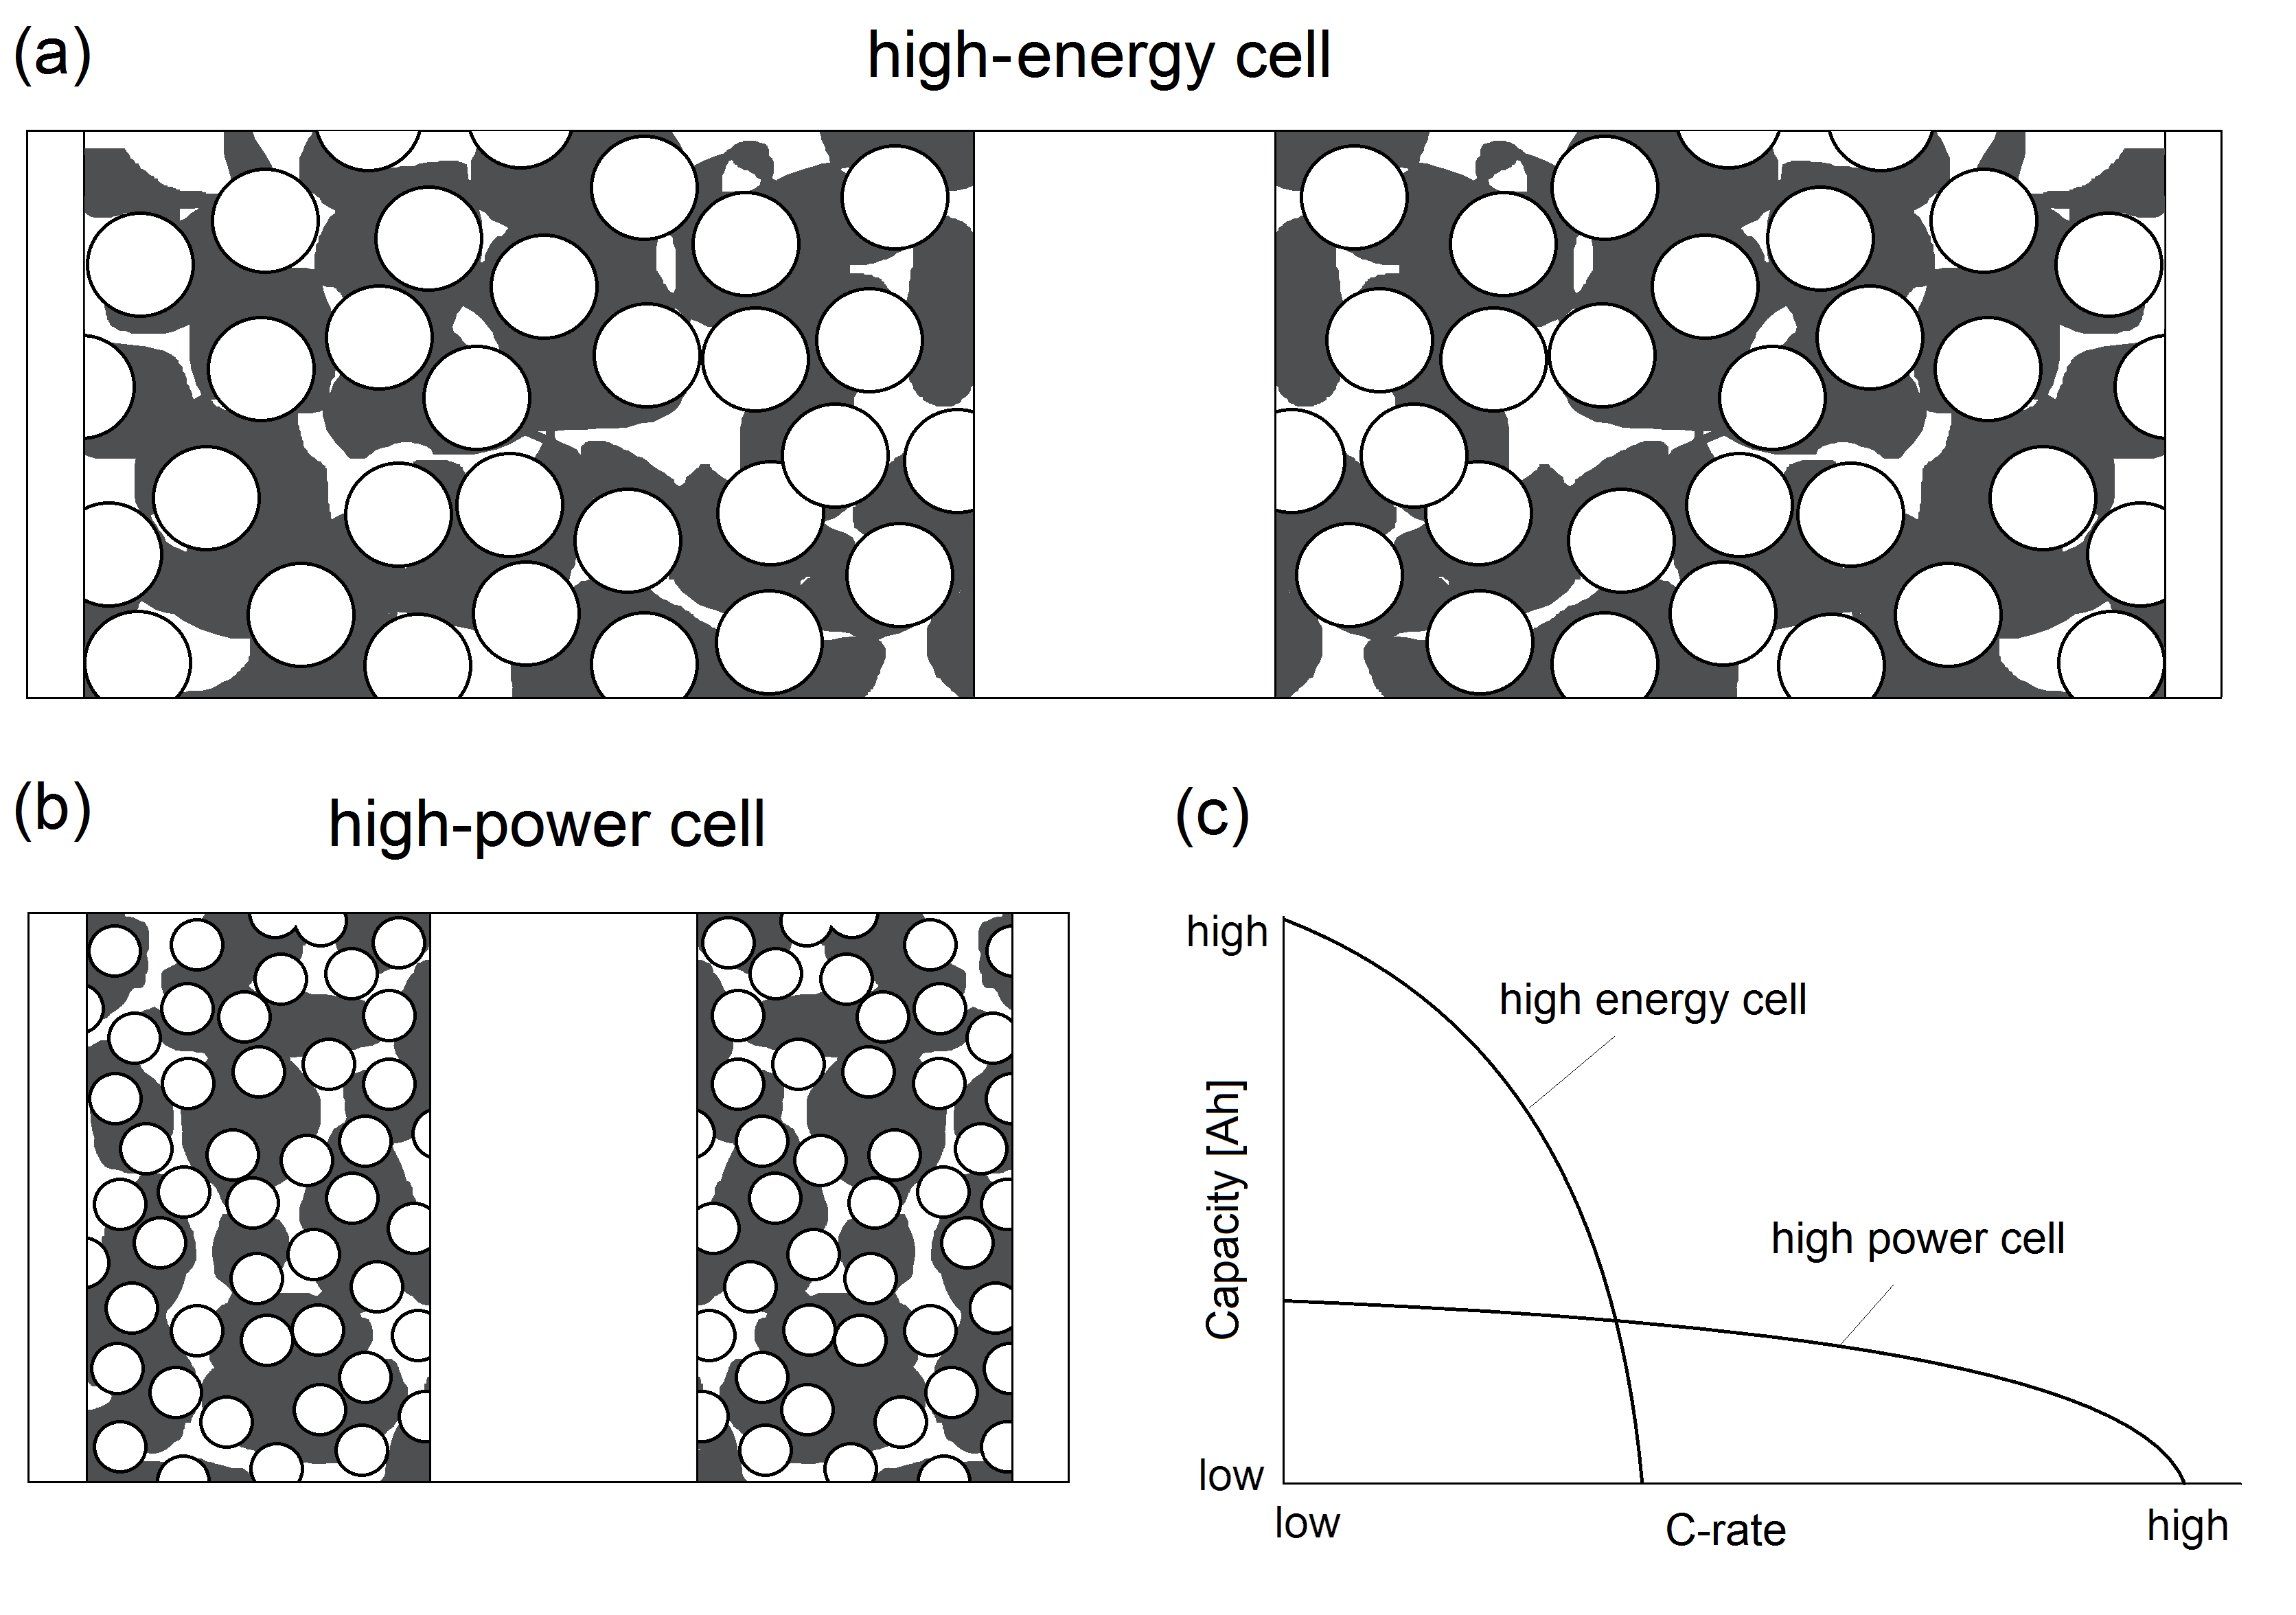
\includegraphics{energy_vs_powercell}
    \caption[%
    Qualitative comparison  of the  construction of one  layer of  a high-energy
    cell versus a high-power cell
    ]%
    {%
        Schematic  depicting a  qualitative  comparison of  the construction  of
        one  layer  of  a  high-energy   cell  versus  a  high-power  cell.  The
        illustration  at top  depicts one  layer of  a high-energy  cell wherein
        thick  electrodes  are  used.  The bottom-left  illustration  depicts  a
        single layer  of a high-power  cell wherein very thin  electrode regions
        are  used.  Both  cell  diagrams  are  drawn  to  the  same  scale.  The
        bottom  right  plot  qualitatively indicates  the  relationship  between
        C-rate  and  the nominal  cell  capacity.  Illustration reproduced  from
        \mbox{von~Srbik~\cite{VonSrbik2015}}

    }%
    \label{fig:energyvspowercell}
\end{figure}


Therefore, there exists  a research question on what constitutes  the best layer
choice  that straddles  this  trade-off  with the  least  penalty  to the  power
capability  of  the  cell  whilst simultaneously  having  the  maximum  possible
capacity. This  saddle point determination needs  to be performed for  a curated
set of power input/output conditions to the cell. This niche problem has not yet
been  tackled by  researchers  and therefore  motivates the  need  to perform  a
careful design study which is documented in this chapter.

\FloatBarrier

\subsection{Quantitative demonstration of energy/power trade-off}\label{sec:energypowertradeoffdemo}

The discussion in \cref{subsec:layeroptmotivation} has motivated the need for an
in-depth exploration of the energy to power trade-off expressed as a function of
the number of  layers. Before embarking on constructing a  framework to optimise
the layer choice by formalising various constraints that govern this optimality,
this section aims to quantitatively  demonstrate this relationship by applying a
fixed galvanostatic discharge to an example cell. Additionally, the crucial idea
of \emph{usable} energy versus \emph{total} stored energy is also introduced.

A  \gls{lco}  cell  whose  physical  properties  and  simulation  parameters  is
drawn from  the combined set of  data from tables~\ref{tbl:lcoSimParamslayeropt}
and~\ref{tbl:lcoSimParamsSPMp2d} is  used as the  example cell. The only  set of
values that overlap between these two tables are ---
\begin{enumerate*}[label=\itshape\alph*\upshape)]
    \item the cut-off voltages, and
    \item the number of nodes  used for numerical  discretisation of  the governing  \gls{pdae} equations.
\end{enumerate*}
For these conflicting quantities,  the values in \cref{tbl:lcoSimParamslayeropt}
prevail for all simulation studies  in this chapter. Furthermore, the individual
electrode thicknesses  from \cref{tbl:lcoSimParamsSPMp2d} is not  directly used,
but  instead  calculated  for  every  layer  choice  by  keeping  the  ratio  of
their  relative  thicknesses  constant.  This   aspect  shall  be  explained  in
\cref{sec:electroderatio}.

\Cref{fig:fig_CC_discharge_curves}  illustrates  the  influence  of  the  number
of  layers   on  the  energy   and  power   capability  of  the   example  cell.
Starting  at  \SI{100}{\percent}  \gls{soc},  a constant  current  discharge  of
\SI{60}{\ampere}\footnotemark{}  is applied  to a  \gls{dfn} model  of the  cell
until reaching the  lower cut-off voltage. For each discharge  run, the model is
reconfigured  with  a  different  layer  choice.  Five  distinct  layer  choices
have  been carefully  conjured so  as  to provide  a clear  illustration of  the
energy/power trade-off phenomenon.

\begin{figure}[!bp]
    \begin{minipage}[t]{\textwidth}
        \centering
        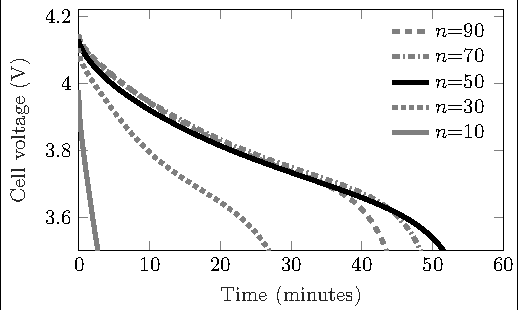
\includegraphics[trim=4 4 2 4,clip]{fig_CC_discharge_curves.pdf}
        \captionsetup{labelsep=note}
        \caption
        [%
        Voltage curves for a \SI{60}{\ampere} galvanostatic discharge from
        \SI{100}{\percent} \glsfmtshort{soc} until cut-off voltage for a few layer
        choices, in a pouch cell of fixed exterior height.
        ]%
        {%
            Terminal voltage curves of a Li-ion cell (with parameters
            given in \cref{tbl:lcoSimParamslayeropt}) under a \SI{60}{\ampere}
            galvanostatic discharge beginning from \SI{100}{\percent}
            \glsfmtshort{soc} until lower cut-off voltage for a few layer
            choices~$n$, in a pouch cell of fixed exterior height. The maximum
            usable energy is achieved for an intermediate choice of $n$
            that corresponds to neither the highest nominal capacity layer
            configuration ($n$=\num{10}) nor the highest electrode surface area
            configuration ($n$=\num{90}).
        }%
        \label{fig:fig_CC_discharge_curves}
        \mpfootnotes[1]
        \footnotetext{{The   rationale  behind  choosing   this  specific
                magnitude  of  applied  current  is   explained  in  the  section  dealing  with
        \hyperlink{refcellselection}{selection of a  suitable reference capacity cell} (also see \cref{sec:surfareaperlayer}).}}

        \footnote{This figure was created by \mbox{Ian Campbell} who asserts copyright,
            with intellectual contributions from and the right to use asserted by
        \mbox{Krishnakumar Gopalakrishnan}.}
    \end{minipage}
\end{figure}

As  seen  in \cref{fig:fig_CC_discharge_curves},  during  the  initial phase  of
discharge, the terminal voltage  of the cell is the highest  for the two highest
layer choices  \ie{} $n  = 90$  and $n=70$. Consistent  with the  explanation in
\cref{subsec:layeroptmotivation}, these  two layer choices have  thin electrodes
and  hence  comparatively low  resistances  leading  to  only a  small  internal
overpotential drop. However,  as expected, their total energy is  lower than the
cell with  $n=50$ layers as  evidenced by  their relative run-times  until lower
cut-off voltage.  This is to  be expected as the  thin electrodes of  these high
layer count cells cannot  store a large volume of active  material. Based on the
explanation  from \cref{subsec:layeroptmotivation},  it  is  expected that  this
trend  will continue  \mbox{\ie{} the}  lower the  layer count,  the higher  the
run-time until  cut-off. If this  were the case,  prima~facie it seems  that the
layer optimisation task is trivial.

Inspecting the discharge curves of lower layer choices brings into limelight the
concept of \emph{usable} energy. Contrary  to expectations, the discharge curves
corresponding  to very  low layer  counts in  \cref{fig:fig_CC_discharge_curves}
terminate even earlier than $n=50$. This is  owing to the fact that although the
total  stored energy  in cells  with low  layer counts  is much  higher, only  a
fraction  of it  is usable.  This  aspects introduces  non-trivial dynamics  (as
discussed below) to an otherwise linear optimisation task.

For  instance,  when $n  =  10$,  the terminal  voltage  of  the cell  collapses
instantaneously, reaching cut-off  voltage whilst its \gls{soc}  remains as high
as \SI{96}{\percent}. At very low layer  counts, the thickness of each electrode
is high. This presents a high resistance  to the flow of charges thereby leading
to  high overpotential  drops  within the  cell. The  usable  energy under  this
\SI{60}{\ampere} galvanostatic  discharge for various layer  choices is compared
in \cref{tbl:CC_discharge_curves_table}. It can be  seen that for very low layer
counts,  the usable  energy that  can be  extracted is  miniscule, albeit  their
theoretical  capacity~$Q_n$  are  in-fact  the highest.  The  usable  energy  in
\SI{}{\watthour} reported in \cref{tbl:CC_discharge_curves_table} is obtained by
multiplying the integral  of the area under each discharge  curve by the applied
current (\SI{60}{\ampere}) with the appropriate scaling of the time-base ( \ie{}
conversion from minutes to hours).

% -*- root: ../../main.tex -*-
%!TEX root = ../../main.tex

\begin{table}[!htbp]
    \caption
    [%
    Theoretical  capacity \&  usable energy  of a  Li-ion cell  for a  few layer
    choices under a \SI{60}{\ampere} galvanostatic discharge
    ]
    {%
        Theoretical capacity and usable energy of a Li-ion cell (with parameters
        given in \cref{tbl:lcoSimParamslayeropt}) for  a few layer choices under
        a \SI{60}{\ampere} galvanostatic discharge.
    }%
    \label{tbl:CC_discharge_curves_table}
    \centering
    \begin{tabular}{@{} S[table-format=2.0] S[table-format=1.2] S[table-format=2.2]  S[table-format=3.2] S[table-format=2.2] @{}}
        \toprule
        \multicolumn{1}{@{} l}{$n$} &  \multicolumn{1}{c}{\footnotesize C-rate} & \multicolumn{1}{c}{\footnotesize \makecell{Theoretical \\ Capacity  (\si{Ah})}} & \multicolumn{1}{c}{\footnotesize \makecell{Usable \\ Energy \si{(Wh)}}} & \multicolumn{1}{c @{}}{\footnotesize \makecell{Remaining \\ SOC  (\si{\percent})}} \\
        \midrule
        90 & 1.24 & 48.25 & 166.46 & 9.84  \\
        70 & 1.11 & 53.99 & 184.80 & 10.26 \\
        50 & 1.00 & 59.73 & 195.47 & 13.51 \\
        30 & 0.92 & 65.47 & 101.20 & 58.95 \\
        10 & 0.84 & 71.21 & 10.15  & 96.22 \\
        \bottomrule
    \end{tabular}
\end{table}


\Cref{tbl:CC_discharge_curves_table}  also brings  into view  the fact  that the
\mbox{C-rate} of the  cell becomes a variable quantity even  for a galvanostatic
discharge,  due to  the dependence  of  its nominal  capacity on  the number  of
layers~$n$. This represents a departure from the norm in the modelling community
wherein the  performance of cells  are quantified as  a function of  the applied
C-rate  \eg{} in  chapters~\ref{ch:spmanalysis} and~\ref{ch:newelectrolytemodel}
of  this thesis.  However, the  preliminary investigation  thus far  has quickly
revealed that  this normalised  quantity does  not hold  much importance  in any
study where the number of layers within a pouch cell is varied.

Taking into account  these factors, a reasonable choice of  the number of layers
in  this specific  \SI{60}{\ampere} galvanostatic  application for  this example
cell  could  be $n=50$.  This  represents  a  practical compromise  between  the
surface area  available for  reaction and  the total  volume of  active material
accommodated.  Out of  the finite  layer configurations  considered, this  layer
choice offers the highest usable energy for the given discharge rate.

In this  sample study, only  a handful of  layer choices were  considered, which
represents  only  a  small  possibility  of  the  overall  design  space  to  be
considered. Furthermore,  thermal considerations were  not explored so  far. For
robust  cell design,  manufacturers  shall need  a  widely applicable  model-led
design tool  that can tackle the  various scenarios that can  occur in real-life
operating conditions. A  deterministic set of optimality criteria  for the layer
selection  is also  to  be formulated.  The choice  $n=50$,  therefore does  not
represent the general optimal layer choice  even for this example cell. However,
this sample study  serves as an illustrative demonstration of  the trade-offs in
energy  versus  power handling  capability  of  a cell  for  a  specific set  of
conditions. Furthermore, it introduces  the complicating aspect of \emph{usable}
capacity into what would have otherwise been a trivial exercise, thereby setting
the tone for the development of a general layer optimisation framework for pouch
cells.



\section{Scope and Context within \glsfmtshort{xeV} Powertrain}
% -*- root: ../../main.tex -*
%!TEX root = ../../main.tex
% vim:textwidth=80 fo=cqt conceallevel=0


It is  important to provide the  contextual setting for this  layer optimisation
work since it is nestled deep  within the broader horizon of electric drivetrain
optimisation. \Cref{fig:fig_PowertrainSchematic}  provides a  graphical overview
depicting the hierarchical architecture of  a typical \gls{xeV} powertrain, from
the  system level  down to  a  single electrochemical  layer. The  rest of  this
section describes the scope of this  layer optimisation work and its integration
into this  overall architecture. A further  set of assumptions that  were deemed
inopportune to be discussed  in \cref{subsec:layeroptassumptions}, is introduced
at apropos junctures  throughout this narrative. The overall  architecture of an
\gls{xeV}  powertrain  can  be  studied through  a  systematic,  hierarchical
evaluation at ---
\begin{enumerate*}[label=\itshape\alph*\upshape)]
    \item the system-level,
    \item the pack-level, and
    \item the cell-level.
\end{enumerate*}

\begin{figure}[!bp]
    \begin{minipage}[t]{\textwidth}
        \centering
        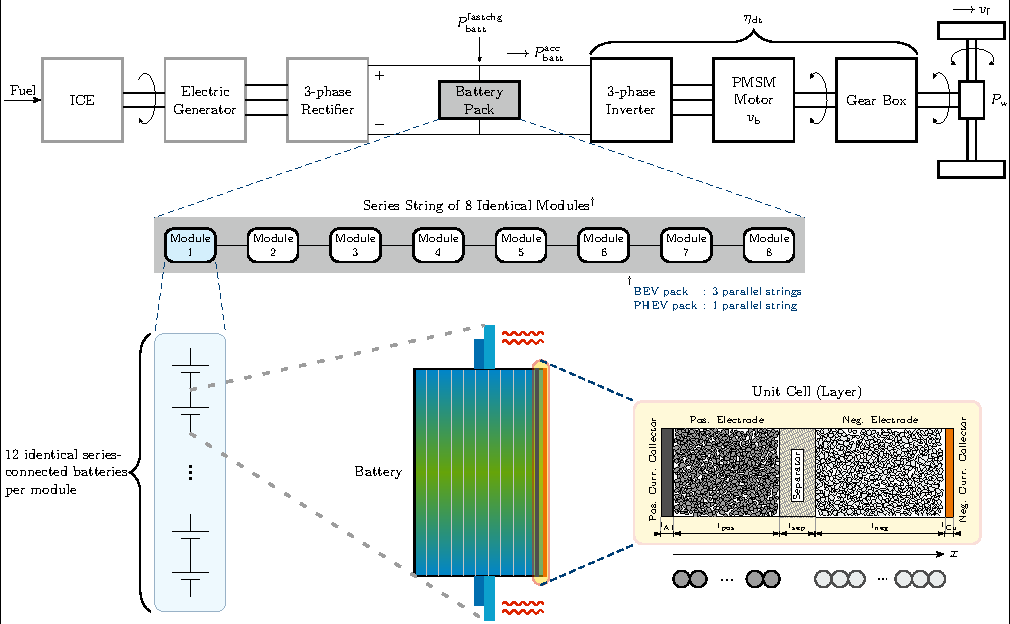
\includegraphics[width=\textwidth]{hierarchical_powertrain_to_cell_layer.pdf}
        \captionsetup{labelsep=note}
        \caption
        [%
        Vehicle-to-cell hierarchical overview of an electrified powertrain architecture
        ]%
        {%
            Schematic depicting the vehicle-to-cell hierarchical overview of
            a typical electrified powertrain architecture. This represents the
            system-level context within which the proposed layer optimisation framework
            has been developed. Two \glsfmtshort{xeV} powertrains ---
            \begin{enumerate*}[label=\itshape\alph*\upshape)]
                \item a \gls{bev}, and
                \item a series \gls{phev}
            \end{enumerate*}
            are chosen as examples to demonstrate how the methodology facilitates
            common module designs for such battery packs.
        }%
        \label{fig:fig_PowertrainSchematic}
        \mpfootnotes[1]
        \footnote{This figure was created by \mbox{Krishnakumar Gopalakrishnan} who
            asserts copyright, with intellectual contributions from and the right to
        use asserted by \mbox{Ian D.\ Campbell}.}
    \end{minipage}
\end{figure}

\subsection{System-level --- vehicular platforms}

The top row of  \cref{fig:fig_PowertrainSchematic} represents the typical layout
of a \emph{series}-hybrid powertrain~\cite{Maksimovic2012}. Partly to supply the
mechanical  power and/or  partly  to  charge the  battery  during propulsion,  a
downsized \gls{ice} is  employed. The \gls{ice} is coupled to  the pack's DC bus
through  a  generator  and  three-phase  rectifier.  While  tackling  the  power
handling  requirements,  irrespective  of  whether  a  \gls{bev}  or  \gls{phev}
powertrain is  being considered, the  cells in the pack  are to be  designed for
the  worst-case operating  scenario \ie~without  any power  support from  the
\gls{ice}. This implies that all discharge  simulations of the \gls{phev} are to
be conducted with  the powertrain operating in all-electric mode  resulting in a
net charge-depletion. The only distinction is that the \emph{magnitude} of power
to  be handled  by the  pack in  this worst  case scenario  is vastly  different
between the \gls{bev} and \gls{phev}  cases. This allows for some simplification
as explained  below and  helps to  narrow down the  scope of  the problem  to be
tackled.

Omitting the  components to the  left of the  battery pack (represented  as text
boxes with light grey border) shall render a powertrain corresponding to that of
a  \gls{bev}.  The proposed  layer  optimisation  methodology is  developed  and
presented in the context of this  \gls{bev} powertrain. However, being a modular
framework, the optimisation methodology may  be readily extended to a \gls{phev}
powertrain.

As  shown   in  \cref{fig:fig_PowertrainSchematic},  the   \gls{bev}  powertrain
typically comprises of ---
\begin{enumerate*}[label=\itshape\alph*\upshape)]
    \item a battery pack,
    \item a three phase inverter,
    \item a \gls{pmsm},
    \item a gearbox for  torque multiplication, and
    \item the rest of the  powertrain  (differential shaft  and driven  wheels).
\end{enumerate*}
Considering the  worst-case scenarios, the  power to  be handled by  the battery
pack arises due to  ---
\begin{enumerate*}[label=\roman*)]
    \item fast charging from  the mains~$P^\text{fastchg}_\text{batt}$~(charge), or
    \item acceleration  from standstill~$P^\text{acc}_\text{batt}$~(discharge).
\end{enumerate*}
The   acceleration  power   is  computed   from  the   power  required   at  the
wheels~$P_\text{w}$.  The   details  of  this  calculation   is  presented  in
\cref{sec:accpathway}.  The  sign  convention  used  in  this  chapter  is  that
the  charging power  is positive  (and  consequently, the  discharging power  is
negative).

\subsection{Pack-level --- strings, modules \& cells}\label{sec:packlevelhierarchy}

Delving  into the  battery pack  under  consideration, this  thesis considers  a
standard  modular  layout wherein  the  \gls{phev}  pack  has one  string  while
the  \gls{bev}  pack  has  three  parallel strings.  Within  each  string,  both
vehicular  platforms employ  8~series-connected  modules.  Taking cognisance  of
the  benefits  of common  module  design,  identical  pack modules  are  assumed
across  both  \gls{xeV}  platforms  which  is  then  extrapolated  to  impose  a
stronger  condition  of  identical  geometry  for  the  constituent  cells  (see
\cref{subsec:layeroptassumptions}). The  exterior dimensions of the  pouch cells
under consideration are listed in \cref{tbl:lcoSimParamslayeropt}.

Each module consists  of 12~identical series-connected cells  denoted by battery
circuit symbols (cyan-filled  blocks in \cref{fig:fig_PowertrainSchematic}). The
\gls{phev} pack is  smaller and consists of only \ordfrac{1}{3}  of the cells in
the \gls{bev} pack. Assuming that the \gls{bev} pack consists of a \mbox{96S-3P}
cell  assembly,  this implies  that  the  \gls{phev}  pack  shall conform  to  a
\mbox{96S-1P} layout. The DC~bus voltage is unaltered since both packs have same
amount of  series cells. The power  flow is assumed to  be uniformly distributed
across all  the cells within  the pack(s). At first,  the power required  at the
terminals of the  pack is computed. From this, a  first-order design ball-parking
of the layers of the cell is made through a single cell simulation. This process
enables reduced simulation run-time with the conditions of one cell assumed to be
representative of all cells in the pack.


% At a  high-level, the  essence of  the layer  optimisation methodology  can be
% distilled down to the following sequence.

While the aforementioned assumption of identical cell conditions across the pack
seems infeasible at first glance, three careful considerations have been made to
justify  this assumption.  Firstly,  power  (and not  current)  is  used as  the
stimulus to the cell. This  implies that, despite the \emph{parallel} connection
of cells  (in groups of three  cells within each module),  each cell experiences
the same  power. Even  across parallel-connected strings,  the power  handled by
each cell shall be the same.  This necessitates the modification of the standard
\gls{dfn}  model in  order to  accommodate power  inputs which  is discussed  in
\cref{sec:innatepowerinput}. Secondly,  although the current  in all cells  of a
\emph{series}  string remain  the same  (by virtue  of Kirchoff's  current law),
their  terminal voltage  levels could  drift away  from each  other and  becomes
unbalanced over  time~\cite{Andrea2010}. This naturally raises  questions on the
assumption  of  identical  conditions  for  all  cells.  However,  this  voltage
unbalance is mitigated with the help of modern \glspl{bms} that employ balancing
techniques  such as  passive  bleeder resistors  or  sophisticated active  dc/dc
converters. Yet another adverse effect that  poses a threat to the assumption of
identical  conditions  is  the  uneven distribution  of  cell  temperatures.  In
automotive packs employing natural convection, cells that are physically located
innermost in  the string tend  to get hotter  than the outermost  cells. Through
good thermal management  design \eg~forced cooling through  circulation of the
coolant through conduits grooved into the pack, thermal balance may be achieved.
Therefore,  it  can be  argued  that,  when  operating  in a  well-designed  and
controlled environment,  cell-to-cell deviations  are minimised.  This justifies
the  global representation  of  all  cells in  the  pack  through a  single-cell
simulation, although modifications to the  simulation model are deemed necessary
to facilitate power inputs.


% Since  thermal effects  need to  be considered  for robust  cell design,

\subsection{Cell-level --- layers, cooling, electrochemical \& thermal models}\label{sec:celllevelxeVinfo}

The    illustration    at     the    centre    of    the     bottom    row    in
\cref{fig:fig_PowertrainSchematic} shows  a schematic  representation of  a cell
arranged within  each module. In practice,  the physical layout of  cells within
a  module  is  slightly  more  complex.  For  instance,  a  typical  arrangement
consists  of  groups   of  3~parallel  cells.  However,   the  illustration  in
\cref{fig:fig_PowertrainSchematic}  suffices to  explain  the necessary  details
required for the specific task at hand.

Each cell in the pack consists of a number of identical layers~$n$. Each layer
consists of ---
\begin{enumerate*}[label=\roman*)]
    \item a~positive current-collector,
    \item a~positive electrode region,
    \item a~separator material,
    \item a~negative electrode region, and
    \item a~negative current-collector.
\end{enumerate*}
Particular attention is called out in  regard to the distribution of temperature
within  the cell.  In  the schematic  of \cref{fig:fig_PowertrainSchematic}  the
shading scheme  is such that greener  tints represent the hotter  regions of the
cell while bluer tints represent colder regions. Furthermore, heat exchange with
the surroundings is also graphically  illustrated through cooling plates mounted
at the tabs  of the cell. This  highlights the specific type  of cooling assumed
\viz~\emph{tab-cooling}  as  opposed to  conventional  \emph{surface-cooling}
historically employed for automotive applications. The assumption of tab-cooling
is an  essential requirement for  upholding the  validity of the  proposed layer
optimisation scheme, and therefore warrants further justification.

An  experimental  study  by   Hunt~\etal~\cite{Hunt2016}  compared  tab  cooling
of  cells  against conventional  surface  cooling.  It  was found  that  \approx
\SI{8}{\percent} increase in the usable  capacity of pristine cells was achieved
with tab cooling relative to that  achieved with surface cooling. Secondly, with
surface  cooling, the  loss rate  of usable  capacity over  thousand cycles  was
nearly thrice of that with tab cooling.  This implies that using tab cooling can
potentially help to extend the lifetime of  the pack by three times. Thirdly, at
higher discharge rates,  surface cooling resulting in a loss  of usable capacity
of \SI{9.2}{\percent} compared  to just \SI{1.2}{\percent} for  tab cooling. The
simulations  discussed  as  part  of  the  optimisation  framework  reported  in
\cref{sec:layeroptframework} are intended to  obtain robust cell designs capable
of handling  worst-case power inputs.  In these  scenarios, tab cooling  is more
appropriate.  Therefore,  this author  has  no  qualms about  recommending  this
specific cooling mechanism  to be used in conjunction with  the results reported
(see  \cref{sec:resultslayeropt}) by  applying the  proposed layer  optimisation
scheme.

Apart  from  its  aforementioned  beneficial   effects  on  cell  longevity  and
performance,  with the  integral  assumption  of tab  cooling,  there exists  an
important side effect  that affects the very  core of the numerics  of the layer
optimisation methodology.  Carefully examining the  shading scheme used  for the
schematic  in the  centre-bottom  of  \cref{fig:fig_PowertrainSchematic}, it  is
clear that  at any vertical  co-ordinate in space  within the cell,  the shading
across the entire cell width remains  uniform throughout. This implies that each
layer  along  a  one-dimensional  cross-section  of the  cell  is  at  the  same
temperature. Based  on the inferences from  Hunt~\etal~\cite{Hunt2016}, with tab
cooling, only  small thermal gradients are  induced in the planar  direction. In
this unique scenario,  the thermal effects within the cell  are not large enough
to warrant a detailed numerical discretisation.  On the other hand, ignoring the
temperature distribution  of the  cell shall  not lead  to robust  cell designs,
especially given  that design simulations  typically involve high  magnitudes of
power.

In  situations akin  to  aforementioned circumstances,  a  lumped thermal  model
of  the cell  has  been  recommended by  Pals  and Newman~\cite{Pals1995}.  This
represents a good trade-off between accuracy and simplicity and hence, is deemed
to  be  appropriate for  this  design  application.  A  suitable value  for  the
convective heat transfer  coefficient~$h$ (see \cref{tbl:lcoSimParamslayeropt}),
comparable  to the  typical  magnitudes in  forced air  convection,  is used  to
represent the heat transfer from the  cell to the environment. The heat exchange
area is the combined  surface area of the two cooling tabs  that are situated at
either end  of the  cell. The temperature  of the coolant  (a thermal  `sink' in
thermodynamic  terminology) is  denoted by~$T_\text{sink}$.  In this  work, this
ambient temperature is held constant during  the course of a simulation run, but
is allowed  to change to  different constant  values between set  of simulations
as  per relevant  vehicle  testing  standards. The  details  of  this aspect  is
discussed  in  \cref{sec:layeroptframework}.  The  material  properties  of  the
constituent components  of each layer  coupled with  the total number  of layers
used  determine  the  lumped  mass  and specific  heat  capacity  of  the  pouch
cell.  These  computations  are  discussed  in  sections~\ref{sec:massofonecell}
and~\ref{sec:spheat} respectively. The  assumption of tab cooling  thus leads to
this qualitative  description of  the lumped  thermal model to  be used  for the
design simulations.  Further quantification by  way of relevant  model equations
and  the computation  of  the constituent  parameters of  the  thermal model  is
embedded as an integral aspect of  the layer optimisation framework and shall be
presented in \cref{sec:spheat}.

As a final observation, all layers  within the cell are electrically in parallel
which implies that their terminal voltages are identical. The current (or power)
at the  cell terminals is  shared equally  among each layer.  The aforementioned
considerations have important  ramifications on the cell modelling  and helps to
drastically  simplify  it. Specifically,  these  considerations  imply that  the
electrochemical  performance  of any  one  layer  is  identical to  every  other
layer.  Therefore,  in conjunction  with  a  lumped  thermal model,  a  standard
\gls{p2d}  discretisation  of  the  \gls{dfn}  model  suffices  to  capture  the
electrochemical behaviour of  the entire cell. The  bottom-right illustration of
\cref{fig:fig_PowertrainSchematic} presents a  one-dimensional discretisation of
the  cell layer  across its  thickness. The  spheres along  the axial  direction
represent computational nodes  wherein the solid-phase diffusion  equation is to
be solved  (see \cref{sec:dfnmodel} for a  brief overview). It is  this standard
\gls{dfn}  model,  suitably  amended  to  accept  power  inputs,  that  will  be
the  backbone of  the  electrochemical  aspects of  the  design simulation.  The
electrochemical model shall be strongly coupled  in a bidirectional sense to the
lumped thermal model  \ie~the temperature of the cell  shall influence various
cell parameters  (see \cref{tbl:lcoSimParamslayeropt}) while  the overpotentials
and currents in  the cell shall play a  role in the rate of  heat generation and
cell temperature simultaneously.

Thus, through a  systematic set of simplifying assumptions  that are justifiable
in a real-world  design, the system-level requirements at the  pack-level can be
suitably  scaled  down  to  power-density  inputs at  the  layer  level.  Having
established the  contextual setting and  scope of  this work within  the broader
landscape of drivetrain  optimisation, it is now possible to  proceed to the set
of numerical enhancements  required to be incorporated into  the \gls{dfn} model
to handle the specific requirements of this layer optimisation task.



\section{Enhancements/Modifications to Standard \glsfmtshort{dfn} Model}
% -*- root: ../../main.tex -*
%!TEX root = ../../main.tex
% vim:textwidth=80 fo=cqt conceallevel=0

\subsection{Augmentation of parameters to standard \glsfmtshort{dfn} model}

\subsubsection*{Cell capacity and electrochemically active surface area}

The  \gls{p2d} implementation  of  the standard  \gls{dfn}  model lacks  certain
parameters that are vital to the  layer optimisation process. The cell's nominal
capacity is a fundamental quantity that gets  altered as the number of layers is
varied. However, it may be surprising  to discover that this parameter is absent
in present  research literature  discussing the  \gls{p2d} model.  The rationale
behind this glaring omission becomes clear  upon closer examination of the model
equations presented in  \cref{tbl:dfneqns}. These equations do not  operate on a
cell level, but  instead operate on a  normalised basis \ie{} only  one layer is
modelled on a  \emph{unit area} basis wherein the stimulus  driving the model is
the applied current  \emph{density} rather than the total  external current. The
layer  optimisation task  here faces  a unique  predicament of  adhering to  the
present modelling paradigm  to retain compatibility with  standard models whilst
still incorporating  the concept of cell's  capacity as a function  of number of
layers.

To  tackle the  aforementioned quandary,  it  is key  to realise  that the  core
parameter  that  varies with  the  number  of layers  in  a  pouch cell  is  the
\emph{electrochemically  active  cross-sectional surface  area}~$A_\text{cell}$.
Curiously, published  literature on  physics-based cell  modelling do  not place
rigorous emphasis on  this key parameter. Most often, to  this author's chagrin,
this  parameter is  simply  listed in  a  standard table  of  parameters and  is
typically  sourced from  a historic  parameter-set with  no further  explanation
provided.

For  a pouch  cell, the  overall electrochemically  active surface  area can  be
defined as
\begin{equation}\label{eq:overallarea}
    A_\text{cell} = n \times A_\text{elec}
\end{equation}
where $n$ is  the number of layers and $A_\text{elec}$  is the electrochemically
active surface area per layer.

\subsubsection*{Surface area per layer}\label{sec:surfareaperlayer}

A literature search reveals that akin  to cell capacity, there is no information
of  cross-sectional geometry  provided in  articles dealing  with the  \gls{p2d}
implementation of  the \gls{dfn} model. To  determine the surface area  per face
(per layer), the author proposes  a new methodology/process involving a sequence
of  steps, based  on  certain  assumptions and  literature  search. The  process
involves  selection of  a  real-world cell,  and ultimately  mapping  it to  the
surface area per  unit face. To the  best knowledge of the  author, this reverse
parametrisation process  (explained next), mapping  from a real-world cell  to a
\gls{p2d} parameter, is  a unique idea and  is claimed as a  contribution to the
art.

\begin{enumerate}[ label=\textbf{\arabic*}), leftmargin=0pt, itemindent=20pt, labelwidth=15pt, labelsep=5pt, listparindent=0.7cm, align=left]
    \item \hypertarget{refcellselection}{\textbf{Selection of a suitable reference capacity cell}}

        Although  this value  shall not  be used  in the  actual layer  optimisation
        procedure itself, this is a  crucial first-step towards obtaining a complete
        parameter set, in particular, to obtain the surface area per layer.

        The focus  of this chapter is  to provide ready-to-use solution  to industry
        extend  with the  aim of  improving  the current  state of  the art  through
        optimal layer configuration  of pouch cells. There is a  clear motivation to
        further increase  cell capacities so as  to maximize driving range,  as laid
        out in the beginning of this chapter (see \cref{sec:layeroptintro}).

        With  this  guiding  principle,  as  a starting  point  towards  choosing  a
        reference capacity cell,  a survey was performed to  identify the production
        \gls{bev}  with  the  highest  driving  range.  As  of  2018,~the  Chevrolet
        Bolt~\gls{bev} bears this distinction  with a range of \SI{383}{\kilo\meter}
        as rated  by the  United States Environmental  Protection Agency  (EPA). The
        specifications of  its battery pack is  listed in Liu~\etal~\cite{Liu2016a}.
        The  battery pack  of  this  vehicle consists  of  288~cells  arranged in  a
        96S-3P configuration, in  agreement with the configuration  discussed in the
        drivetrain  hierarchy  of  \cref{sec:packlevelhierarchy}.

        The    Chevrolet   Bolt    \gls{bev}   pack    has   an    energy   capacity
        of   \SI{60.0}{\kilo\watthour}    with   a    nominal   pack    voltage   of
        \SI{350}{\volt}~\cite{Liu2016a}.  However,  for   this  specific  task,  the
        \si{\amphour} capacity is required. This can be obtained as
        \begin{align}
            \text{\si{\amphour} capacity of Bolt cell} & = \frac{\text{Pack Energy } (\si{\watthour})}{\text{Nominal pack voltage (V)} \times {\text{Number of cells in parallel}}} \\
            {}                                         & = \frac{60000}{350 \times 3} \\
            {}                                         & = \SI{57.14}{\amphour}
        \end{align}

        \begin{itemize}[ leftmargin=10pt, itemindent=15pt, labelwidth=5pt, labelsep=5pt, listparindent=0.7cm, align=left]
            \item \textbf{DC bus voltage and revised cell capacity}

                Even  without  a  dc/dc  boost   converter,  robust  design  of  the
                powertrain during  brown-outs should  allow for  continued operation
                even   with   a  slightly   diminished   DC   bus  voltage   \approx
                \SIrange{4}{5}{\percent} lower than nominal~\cite{Maksimovic2012}.
                Considering a maximum permissible dip of \SI{4}{\percent} in the bus
                voltage \ie{} \SI{336}{\volt}, the cell's capacity may be refined as
                \begin{align}
                    \text{\si{\amphour} capacity of Bolt cell} & = \frac{\text{Pack Energy } (\si{\watthour})}{\text{Lowest pack voltage (V)} \times {\text{Number of cells in parallel}}} \\
                    {}                                         & = \frac{60000}{336 \times 3} \\
                    {}                                         & = \SI{59.52}{\amphour}
                \end{align}

                The reference cell's \si{\amphour} capacity is therefore rounded to
                \textbf{\SI{60}{\amphour}}\footnote{In the interest of maintaining consistency, this computed capacity is
                    retained for the cell used in
                    \crefrange{ch:spmanalysis}{ch:newelectrolytemodel} of this thesis. This also explains the use of \SI{60}{\ampere} for
                    the simulations demonstrating energy/power trade-off of
                    \cref{sec:energypowertradeoffdemo} since this current level corresponds to
                the 1C-rate of the cell.}.

            \item \hypertarget{celllowercutoff}{\textbf{Lower cutoff voltage for cells}}

                In  this  layer  optimisation  work, following  the  assumptions  of
                \cref{subsec:layeroptassumptions},  the  overall pack  configuration
                remains  unchanged  and  independent   of  layers  within  a  pouch.
                This  implies that  the undervoltage  threshold for  DC bus  voltage
                throughout  this   work  shall  remain  fixed   at  \SI{336}{\volt}.
                Therefore, with  96~series connected  cells in  a string,  the lower
                cut-off voltage for an  individual cell is \textbf{\SI{3.5}{\volt}}.
                This  value is  reported in  \cref{tbl:lcoSimParamslayeropt} and  is
                used as a termination condition  for all simulations as explained in
                \cref{sec:layeroptframework}.

        \end{itemize}

    \item \textbf{Computation of electrochemically overall active surface area for reference cell}

        For             the            cell             properties            in
        \crefrange{tbl:lcoSimParamsSPMp2d}{tbl:lcoSimParamslayeropt},        the
        majority                of                 parameters                are
        sourced           from          Subramanian~\etal~\cite{Subramanian2009}
        and                Northrop~\etal~\cite{Northrop2011}.                In
        Northrop~\etal~\cite{Northrop2011},  the   \emph{current  density}  that
        corresponds to  a 1C-rate discharge  of a  cell with this  parameter set
        is  reported to  be \approx  \SI{30}{\ampere\per\meter\squared}. In  the
        author's carefully  designed numerical simulations (very  slow discharge
        at C/500 from fully charged state until charge depletion), this value is
        refined to \SI{29.23}{\ampere\per\meter\squared}.

        The task of determining the electrochemically active overall surface
        area of the reference cell is now straightforward
        \begin{align}
            \text{Overall surface area of reference cell}, A_\text{refcell} &= \frac{\text{Cell capacity (\si{\amphour})}}{\text{1C-rate density (\si{\ampere\per\meter\squared})}} \\
                                                                            &= \frac{60}{29.23} \\
                                                                            &= \SI{2.053}{\meter\squared}
        \end{align}

        This  value  is  listed  in  \cref{tbl:lcoSimParamsSPMp2d}  for  use  in
        \crefrange{ch:spmanalysis}{ch:newelectrolytemodel},  but  is  \emph{not}
        used  in  this  layer  optimisation   work.  This  is  because,  as  the
        number  of  layers change,  the  overall  surface  area changes  as  per
        \cref{eq:overallarea}.

    \item \textbf{Setting the pouch height for the reference cell}

        Although the  official press release~\cite{GMBoltBatteryDims}  from the
        manufacturer  of this  \gls{bev} contains  data on  the cross-sectional
        geometry  of the  cell,  it does  not report  its  height. Hence,  this
        information  needs to  be assumed  by extrapolation  from an  alternate
        source wherein the conditions are similar and therefore, can be applied
        for this reference cell.

        The  review   article  by   Gr\"oger~\etal~\cite{Groger2015}  discusses
        various    states    of    the    art   in    energy    densities    of
        electrode   materials  used   in  various   lithium  ion   chemistries.
        At   the   time   of   its   publication,   the   areal   capacity   of
        cells  were  \approx  \SI{2.0}{\milli\amphour\per\centi\meter\squared}.
        These    authors   recommended    an   areal    capacity   target    of
        \SI{4.0}{\milli\amphour\per\centi\meter\squared} for  future automotive
        applications. This  publication also  considers the aspect  of stacking
        layers  into  pouches  of  certain  geometries.  In  particular,  table
        \romanletter{4}  of Gr\"oger~\etal~\cite{Groger2015}  considers a  pouch
        of  \SI{10}{\milli\meter} height,  for which  the aforementioned  areal
        capacities were calculated.

        In       the        case       of       the        reference       cell
        under       consideration,       the      areal       capacity       is
        \begin{equation}
            \text{Areal capacity of reference cell } = \frac{\SI{60000}{\milli\amphour}}{\SI{20527}{\centi\meter\squared}}  = \SI{2.92}{\milli\amphour\per\centi\meter\squared}
        \end{equation}
        which is close  to the desired value in automotive  applications as per
        the recommendations  in Gr\"oger~\etal. Considering that  the reference
        cell is  drawn from  the high energy  density Chevrolet  Bolt \gls{bev}
        cell,  a pouch  height of  \SI{10}{\milli\meter} is  justifiable for
        this task  and is  reported in \cref{tbl:lcoSimParamslayeropt}.  As per
        the assumptions discussed in \cref{subsec:layeroptassumptions}, this is
        held constant throughout the layer optimisation process.

    \item \hypertarget{stackthickness}{\textbf{Compute stack thickness of reference cell}}

        In a  pouch of given height,  the available space to  accommodate layers
        therein is restricted  by a number of factors. For  instance, the wiring
        from the  current collectors  to the tabs,  protective elements  such as
        fuses etc.\ consume space. For instance, the pouch material itself has a
        finite  thickness  and  hence  after  accounting  for  this,  the  stack
        thickness  available  for  layer  placement  is  lower  than  the  pouch
        thickness.
        \begin{align}
            \text{Stack thickness}, L_\text{stack} & = \text{Pouch height} - 2\times \text{pouch thickness} \\
            \text{Stack thickness}, L_\text{stack} & = H_\text{pouch} - 2 T_\text{pouch} \\
            L_\text{stack}(\si{\milli\meter})      & = 10.0 - 2\times(\num{160e-3}) \\
            L_\text{stack}                         & = \SI{9.68}{\milli\meter}
        \end{align}

        The value of stack thickness of  the reference cell is held constant for
        all layer choices used throughout the entire layer optimisation process.

    \item \textbf{Determination of number  of layers within  reference cell}

        The  next  step  is  to  determine  the  number  of  layers  within  the
        reference pouch  cell~$n_\text{refcell}$.

        The thickness of a complete electrochemical sandwich multiplied by the
        number of layers yields the total stack height
        \begin{equation}\label{eq:stackheightrefcell}
            n_\text{refcell}\, (l_\text{Al} + l_\text{pos} + l_\text{sep} + l_\text{neg} + l_\text{Cu}) = L_\text{stack}
        \end{equation}

        The product of  layers and the thickness of  an electrochemical sandwich
        cannot exceed the  overall stack height. This implies  that the equality
        in \cref{eq:stackheightrefcell} is  to be changed to  an inequality with
        the upper  bound of the  computation on the  \gls{lhs} set to  the stack
        height.
        \begin{align}
            n_\text{refcell}\, (l_\text{Al} + l_\text{pos} + l_\text{sep} + l_\text{neg} + l_\text{Cu}) & \le L_\text{stack} \\
            n_\text{refcell}                                                                            & \le \frac{L_\text{stack}}{l_\text{Al} + l_\text{pos} + l_\text{sep} + l_\text{neg} + l_\text{Cu}}\label{eq:stackheightrefcellmod}
        \end{align}

        Since fractional layers do not have  any physical meaning, the number of
        layers that  can be  accommodated within  any pouch  must be  an integer
        quantity. Therefore,  $n_\text{refcell}$ is  computed as the  `floor' of
        the quantity in the \gls{rhs} of \cref{eq:stackheightrefcellmod}
        \begin{align}
            n_\text{refcell} &= \floor*{\frac{L_\text{stack}}{l_\text{Al} + l_\text{pos} + l_\text{sep} + l_\text{neg} + l_\text{Cu}}} \\
            {} &= \floor*{\frac{9.68}{(15 +  72 + 25 + 88 + 10) \times 10^{-3}}} \\
            n_\text{refcell} &= 46
        \end{align}

        The reference cell is thus deemed to consist of 46~layers.

    \item \textbf{Computation of surface area per layer}

        Substituting  the values  of  $n_\text{refcell}$ and  $A_\text{refcell}$
        into  \cref{eq:overallarea}, the  electrochemically active  surface area
        per layer is obtained as
        \begin{align}
            A_\text{elec} & = \frac{A_\text{refcell}}{n_\text{refcell}} \\
            {}            & = \frac{\SI{2.053}{\meter\squared}}{46}     \\
            {}            & = \SI{44.63}{\milli\meter\squared}
        \end{align}

        The   surface   area   per   layer    thus   computed   is   listed   in
        \cref{tbl:lcoSimParamslayeropt} and  is held constant  throughout across
        all  layer choices  tried during  the layer  optimisation process.  This
        assumption  is  immediately  justifiable   from  a  physical  viewpoint,
        since  the process  of assembling  layers is  along the  axial thickness
        direction (aligned with  pouch height) and is independent  of the planar
        (cross-sectional) direction.

\end{enumerate}

\subsection{Modification of standard \glsfmtshort{dfn} model to handle power inputs}\label{sec:innatepowerinput}

As  discussed  in  \cref{sec:packlevelhierarchy}, for  assuming  identical  cell
conditions during operation necessitates that the external stimulus to the cells
is an applied power  value. The cell's terminal voltage as  well as current draw
can be viewed as a response to  this power input. To simulate this condition for
achieving a model-based optimal layer design, the standard \gls{dfn} model which
conventionally handles  current stimuli  has to be  suitably modified  to accept
power inputs.

Plett~\cite{Plett2016}  suggests  a methodology  for  applying  power inputs  to
equivalent  circuit models  simulated  at  a fixed  sample  rate. This  involves
converting the input  power~$P_k$ to a current~$I_k$ using  an equivalent series
resistance~$R_0$. The value of $R_0$ is  updated at every time index~$k$, as per
\cref{eq:PlettPower}. $v_k$ is the cell's terminal voltage at present time
sample $k$, which has been evolved from the  applied current up to and including
the previous  time step $(k-1)$.
\begin{equation}\label{eq:PlettPower}
    I_k = \frac{v_k - \sqrt{v^\text{2}_k - 4R_0P_{k}}}{2R_0}
\end{equation}

There are two disadvantages in using  Plett's simplified approach for this layer
optimisation  study.  Firstly,  this  necessitates  the  quantification  of  the
electrical resistance  of a \gls{pbm}. Such  an idea is at  loggerheads with the
fundamental  philosophy of  \glspl{pbm}  which strive  to  represent a  detailed
picture  of  underlying  phenomena,  as opposed  to  the  system-level  terminal
behavioural characterisation  facilitated by the \glspl{ecm}.  Translating power
to current  in this manner also  necessitates a two-pass conversion  between the
physical  domain and  the electrical  domain ---  a process  likely to  diminish
modelling  fidelity significantly.  Since the  results from  application of  the
model shall inform the number of layers  to be used in a real-world cell design,
such loss of  fidelity is unacceptable. Secondly, the constraint  of using fixed
time interval  updates implies that  a high-speed adaptive  time-stepping solver
cannot be used for handling this power input condition. This shall slow down the
simulation speed considerably since the search space of layer combinations to be
considered is  fairly large.  Furthermore, the simulations  have to  be repeated
over  multiple combinations  of  initial and  ambient  temperatures which  shall
render the model-based design approach to  be too slow and offset its advantages
over a conventional prototype-based design.

Dees~\etal~\cite{Dees2002}  identified the  requirement  of  having a  \gls{p2d}
model that  can run on applied  power. However, in the  aforementioned work, the
relevant  equations for  reformulation  of solid-phase  boundary conditions  are
not  presented. This  thesis  author  therefore feels  compelled  to provide  an
independent derivation of reformulating the \gls{p2d} model to facilitate innate
power input capability. Since the equations  are derived for a single layer, the
power  \emph{density}, obtained  by scaling  the  applied power  by the  overall
active cross-sectional area~$A_\text{cell}$ is used as the driving input.

In  the  \gls{p2d}  model,  charge  conservation in  solid  phase  is  given  by
\cref{eq:solidchargeconserve},  which is  revisited  below.  The subsequent  two
equations pertain to the corresponding  boundary conditions. In these equations,
current density~$i$ represents the applied input.
\begin{align}
    \frac{\partial}{\partial x} \left(\sigma_{\text{eff}} \frac{\partial \phi_\text{s}(x,t)}{\partial x} \right) &= a_\text{s} F j(x,t) \tag{\cref{eq:solidchargeconserve} revisited}\\
    \sigma_{\text{eff}} \frac{\partial \phi_\text{s}(x,t)}{\partial x} \bigg|_{\substack{x_\text{pos/Alcc}\\x_\text{neg/Cucc}}} &= -i\label{eq:solidchargeconservecurrBC}\\
    \sigma_{\text{eff}} \frac{\partial \phi_\text{s}(x,t)}{\partial x} \bigg|_{\substack{x_\text{pos/sep}\\x_\text{neg/sep}}} &= 0
\end{align}

Now,  \cref{eq:undiscretisedPhiSpowerBC}  replaces  the boundary  condition  in
\cref{eq:solidchargeconservecurrBC}  to use  the  applied  power density~$p$  to
drive the model.

\begin{equation}\label{eq:undiscretisedPhiSpowerBC}
\sigma_{\text{eff}_\text{neg}} \left( \phi(x,t) \frac{\partial
\phi_\text{s}(x,t)}{\partial
x}\right)\Bigg\rvert_{\mathrlap{x=x_\text{neg/Cucc}}}  -
\sigma_{\text{eff}_\text{pos}} \left( \phi(x,t) \frac{\partial
\phi_\text{s}(x,t)}{\partial x} \right)\Bigg\rvert_{\mathrlap{x=x_\text{pos/Alcc}}} = p
\end{equation}

\Crefrange{eq:ctspowerconstraint}{eq:cellpositivity}  represent the  constraints
pertaining to physical laws and are  fully satisfied in this case.
\begin{align}
	vi  - p & = 0 \label{eq:ctspowerconstraint} \\
	v       & > 0 \label{eq:cellpositivity}
\end{align}
\Crefrange{eq:undiscretisedPhiSpowerBC}{eq:cellpositivity} are  then discretised
for numerical implementation.

\Cref{fig:1d_fv_mesh}  describes  a  schematic  overview  of  a  one-dimensional
cell-centred  \gls{fv}  discretisation scheme.  Here,  evenly  spaced nodes  are
considered to form  the support mesh along the through-thickness  dimension of a
layer. Vertical  lines denote the  edges of  control volumes whereas  the filled
dots  denote computational  nodes  where the  variables from  \cref{tbl:dfneqns}
pertaining to the axial direction are solved.

\begin{figure}[!htbp]
    \centering
    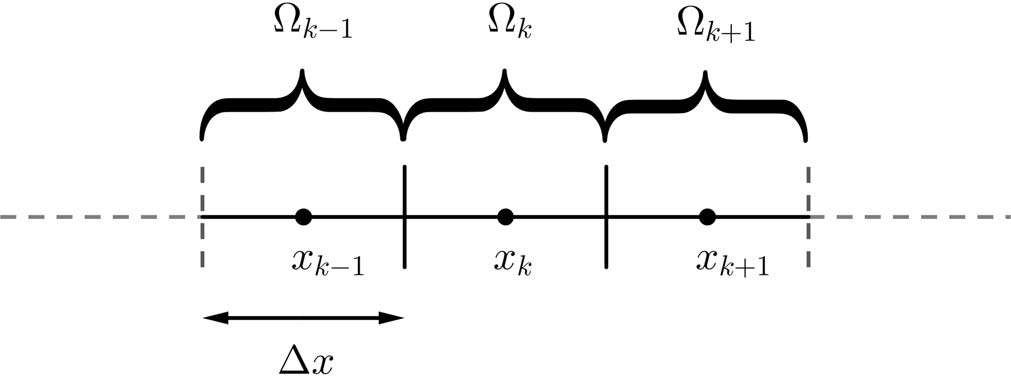
\includegraphics{fv_disc.jpg}
    \caption[Illustration of a standard cell-centred \gls{fv} discretisation
    scheme]{Simplified illustration of a standard cell-centred \gls{fv}
    discretisation scheme. Image reproduced from
Torchio~\etal~\cite{Torchio2016}.}
    \label{fig:1d_fv_mesh}
\end{figure}

\Cref{eq:discretisedPhiS}      represents       the      weak       form      of
\cref{eq:solidchargeconserve} used on the \gls{fv}  mesh in each control volume,
wherein subscripts~$k$ and  $k\pm\frac{1}{2}$ denote the $k$\textsuperscript{th}
\gls{fv} node and its associated left and right edges respectively.
\begin{equation} \label{eq:discretisedPhiS}
    \sigma_{\text{eff}} \frac{\partial \phi_\text{s}(x,t)}{\partial x}\Bigg|_{x_{k-\frac{1}{2}}}^{x_{k+\frac{1}{2}}} = a_\text{s} F j_k(t) \Delta x
\end{equation}

At this juncture, a simplifying approximation for the solid-phase potentials can
be considered. In the standard \gls{fv} scheme, the solution values at the faces
(edges of  control volumes) is  obtained by  interpolating from the  two nearest
\gls{fv} node values. At the two  extrema, a linear extrapolation from the first
and last nodes can be considered.  Accounting for this increases the accuracy of
computations  thereby  providing  good  estimates of  solid  potentials  at  the
interfaces. However, this comes at the  penalty of a more mathematically complex
set of boundary  conditions. When using high node densities  in the negative and
positive electrode  regions (see  \cref{tbl:lcoSimParamslayeropt}), for  the two
outermost control  volumes, the  values of  $\frac{\Delta x}{2}$  becomes small.
With a reasonably small mesh interval, the potentials at the cell centres can be
considered to be  nearly equal to that at their  corresponding current collector
interfaces. This assumption helps to keep the resulting mathematical expressions
tractable.

Applying    \cref{eq:discretisedPhiS}    to    the    first    control    volume
(0\textsuperscript{th} node) in  the positive electrode and to  the last control
volume (n\textsuperscript{th} node) in the negative electrode,
\begin{align}
	\frac{-\sigma_{\text{eff}_\text{pos}} \phi_{\text{s}_0}}{\Delta x_\text{pos}} + \frac{\sigma_{\text{eff}_\text{pos}} \phi_{\text{s}_1}}{\Delta x_\text{pos}} + i &= a_{\text{s}_\text{pos}} F j_0 \Delta x_\text{pos}\label{eq:PhiSappliedBCpos}\\
	\frac{-\sigma_{\text{eff}_\text{neg}} \phi_{\text{s}_n}}{\Delta x_\text{neg}} + \frac{\sigma_{\text{eff}_\text{neg}} \phi_{\text{s}_{n-1}}}{\Delta x_\text{neg}} - i &= a_{\text{s}_\text{neg}} F j_n \Delta x_\text{neg}\label{eq:PhiSappliedBCneg}
\end{align}

Subtracting  the resulting  equations of  multiplying \cref{eq:PhiSappliedBCpos}
with $\phi_{\text{s}_0}$ and \cref{eq:PhiSappliedBCneg} by $\phi_{\text{s}_n}$
\begin{multline} \label{eq:pinputBCcomplete}
    \frac{-\sigma_{\text{eff}_\text{pos}} \phi^2_{\text{s}_0}}{\Delta x_\text{pos}} -
    \frac{\sigma_{\text{eff}_\text{neg}} \phi^2_{\text{s}_n}}{\Delta x_\text{neg}} +
    \frac{\sigma_{\text{eff}_\text{pos}} \phi_{\text{s}_0} \phi_{\text{s}_1}}{\Delta x_\text{pos}} +
    \frac{\sigma_{\text{eff}_\text{neg}} \phi_{\text{s}_n} \phi_{\text{s}_{n-1}}}{\Delta x_\text{neg}} \\+ p -
    a_{\text{s}_\text{pos}} F j_0 x_\text{pos} \phi_{\text{s}_0} - a_{\text{s}_\text{neg}} F j_n x_\text{neg}
    \phi_{\text{s}_n} = 0
\end{multline}
\Cref{eq:pinputBCcomplete} therefore  represents the boundary condition  for the
solid phase  potential \gls{pde} could  be applied to either  electrode, thereby
facilitating the application of an input power density to the \gls{p2d} model.


%%Figure showing power input

\subsection{Hybrid spectral-\glsfmtshort{fv} scheme}\label{sec:hybridfv-spectral}

Fast  and  accurate  estimation  of   the  solid  phase  lithium  concentration,
particularly  its   value  at   the  surface  of   electrode  particles   is  an
inherent  requirement   of  the   layer  optimisation  procedure   presented  in
\cref{sec:layeroptframework}.   The  high   power  densities   to  be   handled,
particularly  at  low   layer  counts  necessitate  this   requirement.  It  has
been   acknowledged  that   solid-phase  concentration   calculations  employing
polynomial    approximations   lack    fidelity    at   high    charge/discharge
rates~\cite{Santhanagopalan2006}.  Hence,  a  conventional  full-order  solution
based on Fick's law of diffusion is required for this layer optimisation task.

With full-order  solid phase  diffusion dynamics,  applying the  \gls{fv} scheme
(that has been  employed in LIONSIMBA~v1.0x to  discretise all through-thickness
\gls{pde}s of the \gls{p2d} model) results  in a very large system of equations.
This is due to the requirement of using a high radial node density per spherical
particle for improved accuracy. Consequently, the computational cost is high and
simulation  runtime  becomes prohibitive  when  exploring  the search  space  of
all  possible  layer configurations.  Moreover,  with  a cell-centered  \gls{fv}
discretisation,  it is  non-trivial to  directly apply  the ionic  flux boundary
condition at the particle surface, since it involves extrapolation from at least
two other nodes within the particle. While such extrapolations are acceptable in
the axial  dimension --- particularly  with high node densities  providing small
values of $\frac{\Delta x}{2}$ --- they are undesirable in the radial dimension.
This  is because  cell's  open  circuit and  terminal  voltages strongly  depend
on  the  concentration  at  the  particle  surface.  Spectral  methods  offer  a
combination  of high  accuracy and  speed while  permitting the  use of  a lower
number  of radial  discretisation nodes.  To implement  a spectral  scheme on  a
non-periodic  domain,  a  Chebyshev discretisation~\cite{Trefethen2000}  may  be
applied.  Bizeray~\etal{}~\cite{Bizeray2015} discretised  all  of the  \gls{p2d}
model  equations using  this approach.  However, this  entails a  bi-directional
mapping of all  variables between the physical and  Chebyshev domains, incurring
computational overhead.

In this chapter, a hybrid formulation of the \gls{p2d} model is proposed wherein
a standard \gls{fv} scheme  in the axial dimension and a  spectral scheme in the
radial domain  are used.  Exploiting this  natural separation  of the  axial and
radial domains enables to ---
\begin{enumerate*}[label=\roman*)]
    \item retain  the   ability  to  easily   couple  the   molar  flux  density   at  the particle  surface  through  reformulation  of the  boundary  conditions  of  the solid  diffusion \gls{pde},  and
    \item solve  for  solid-phase  lithium  concentration  in  the  Chebyshev  domain  and locally transform  to physical  domain, without requiring  system-wide Chebyshev reformulations.
\end{enumerate*}
Although the proposed implementation does  not \emph{globally} employ a spectral
scheme, the  combined beneficial  effects of  radial-domain spectral  scheme and
automatic differentiation of system equations using CasADi~\cite{Andersson2013b}
facilitates rapid simulation, enabling  layer optimisation on short time-scales.
\Crefrange{eq:defineChebNodes}{eq:solidDiffEqChebDomain}   detail  the   steps
leading to  the reformulated solid  phase diffusion and its  associated boundary
condition in the Chebyshev domain.

The $N_\text{r}$~Chebyshev collocation nodes, defined on a 1D mesh in the radial
direction, are given by \cref{eq:defineChebNodes}~\cite{Trefethen2000}.
\begin{equation}\label{eq:defineChebNodes}
    \widetilde{r} = \cos\left(\frac{i\pi}{N_\text{r}}\right), \qquad i = 0, 1, \dots N_\text{r} \quad \widetilde{r} \in [-1, 1]
\end{equation}

Assuming  constant diffusivity,  and expanding  the derivative  in the  standard
form of  the Fickian  spherical diffusion equation  (see \cref{eq:dfnsoliddiff})
for  each particle,  we  obtain  \cref{eq:quotientappliedpde}, presented  along
with  its   Neumann  boundary   conditions \cref{eq:quotientappliedpdeBCcentre}
and \cref{eq:quotientappliedpdeBCsurface}.  $j$~is   the  molar   flux  density
(\si{mol.m^{-2}.s^{-1}}) and $R_\text{p}$ is the particle radius (\si{m}).
\begin{subequations}\label{eq:quotientappliedpde}
    \begin{align}
        \frac{\partial c_\text{s}}{\partial t} &= D^\text{eff}_\text{s} \left( \frac{\partial}{\partial r} \frac{\partial c_\text{s}}{\partial r} + \frac{\partial^2 c_\text{s}}{\partial r^2} \right) \qquad r \in [0, R_\text{p}]\tag{\ref*{eq:quotientappliedpde}}\\
        \diffp{c_\text{s}}{r}{\mathrlap{r = 0}} &= 0\label{eq:quotientappliedpdeBCcentre}\\
        D^\text{eff}_\text{s}\diffp{c_\text{s}}{r}{\mathrlap{r = R_\text{p}}} &= -j\label{eq:quotientappliedpdeBCsurface}
    \end{align}
\end{subequations}

Mapping $r \in [0,R_\text{p}] \mapsto \widetilde{r} \in [-1, 1]$,
\begin{equation}\label{mappingChebDomain}
    r = \frac{R_\text{p}}{2}(\widetilde{r} + 1)
\end{equation}

Applying \cref{mappingChebDomain} to
\crefrange{eq:quotientappliedpde}{eq:quotientappliedpdeBCsurface} whilst
retaining $c_\text{s}$ in the physical space yields
\crefrange{eq:solidDiffEqChebDomain}{eq:solidDiffEqChebDomainBCsurface}.

\begin{subequations}\label{eq:solidDiffEqChebDomain}
    \begin{align}
	    \frac{\partial c_\text{s}}{\partial t}                         & = 4 \frac{D^\text{eff}_\text{s}}{R_\text{p}^2} \left( \frac{2}{\widetilde{r} + 1} \frac{\partial c_\text{s}}{\partial \widetilde{r}} + \frac{\partial^2 c_\text{s}}{\partial {\widetilde{r}}^2} \right)\tag{\ref*{eq:solidDiffEqChebDomain}} \\
        \diffp{c_\text{s}}{\widetilde{r}}{\mathrlap{\widetilde{r}=-1}} & = 0\label{eq:solidDiffEqChebDomainBCcentre}                                                                                                                                                                                                                \\
        2 \frac{D^\text{eff}_\text{s}}{R_\text{p}} \diffp{c_\text{s}}{\widetilde{r}}{\mathrlap{\widetilde{r}=1}} & = -j\label{eq:solidDiffEqChebDomainBCsurface}
    \end{align}
\end{subequations}

During  the iterative  solution process,  the spatial  gradients of  solid phase
lithium concentration  in \cref{eq:solidDiffEqChebDomain}  in this case  are not
computed through  an explicit  differentiation procedure  as usual,  but instead
evaluated by pre-multiplying  the concentration values at  the collocation nodes
by a Chebyshev differentiation matrix. This particular aspect is responsible for
the inherent reduction of simulation  runtime achieved by introducing a spectral
method. In the updated version  of LIONSIMBA~v2.0 (created specifically for this
layer  optimisation work),  differentiation matrices  of suitable  dimensions as
well as the Chebyshev collocation nodes  are generated using the MATLAB function
\texttt{cheb.m}~\cite{Trefethen2000}.

%\subsection{Modelling Platform and Preconditioning}

%Couple of statements  about why LIONSIMBA was chosen as  the modelling platform
%for implementing the p2d dynamics. The  cell parameters used are shown in table
%xx. This cell is henceforth known as the LIONSIMBA cell or Northrop cell.

%Discuss the  missing elements  in LIONSIMBA  only with  respect to  the present
%problem at hand, \viz{the stoichiometries}.

%\subsubsection*{Stoichiometry Augmentation}

%Discuss the problem first. How LIONSIMBA started always at 85.51 percentage and
%needed to  do a  discharge down to  zero percent before  having the  ability to
%charge. For this project, stoichiometries  are vital for capacity determination
%and  the 1C  current density.  Explain how  stoichiometries were  refined until
%cut-off for  infinitesimal bleeding discharge current  achieved. Noted relevant
%values. Explain refinement  of how approximate capacities  reported by Northrop
%and Subramanian were  refined precisely. Explanation of  remnant capacities and
%stoichiometries computation. Explanation of  1C current density.parameters init
%capacity computation code.

%\subsection{Layer Assembly within Pouch Cells}
%With  the  help  of  Northrop's   layer  assembly  figure,  explain  the  layer
%configuration/arrangement within a pouch cell. The next task is then identified
%as computing the number of layers within the reference pouch cell.

%\subsubsection*{Number of Layers of LIONSIMBA aka Northrop cell}
%Krishna came up with the idea of using integer optimisation for this task. The
%software MIDACO was also selected by Krishna and explained to Ian. The MIDACO
%result of the number of layers within the standard cell was now available.

%\subsubsection*{Computation of Surface Area per face, \protect{$A_\text{cell}$}}
%Show the simple algebraic computation of overall surface area $A$ and the
%per-face area $A_\text{cell}$. Explain how the area per face shall be a key
%quantity in the layer optimisation framework discussed later on.

%Layerphoto showing face areas and anode/cathode verhand etc will be shown here

%This concludes the augmented set of parameters added by the author to the basic
%parameter set  of the DFN  model. The added  numerical value of  parameters are
%summaried in table xx. Lots The layer optimisation framework and assumptions is
%described next.



\section{Computational Framework}\label{sec:layeroptframework}
% -*- root: ../../main.tex -*
%!TEX root = ../../main.tex
% vim:textwidth=80 fo=cqt conceallevel=0

% \afterpage{\clearpage}

\subsection{Introduction and guidelines for flow diagram traversal}

The  methodology adopted  by the  proposed layer  optimisation framework  can be
explained by  using the  flow diagram in  \cref{fig:fig_strategy_schematic}. The
power  handled by  the cell  during normal  operation (evaluated  by considering
various drivecycles)  is much  lower than  that experienced  during acceleration
(discharge)  and  fast-charging (charge)  scenarios.  \Cref{sec:resultslayeropt}
provides  a brief  summary of  the peak  and median  powers across  all standard
drivecycles. Therefore, from a design  perspective, it is sufficient to consider
the power  requirements for  these two  extreme cases.  Hence, the  schematic in
\cref{fig:fig_strategy_schematic} can  be studied  by broadly dividing  the flow
diagram into two parts ---
\begin{enumerate*}[label=\roman*)]
    \item an acceleration pathway (primarily consisting of blocks shaded in grey), and
    \item a fast-charging pathway (predominantly composed of blocks shaded in cyan).
\end{enumerate*}

\begin{figure}[p]
    \begin{minipage}[t]{\textwidth}
        \centering
        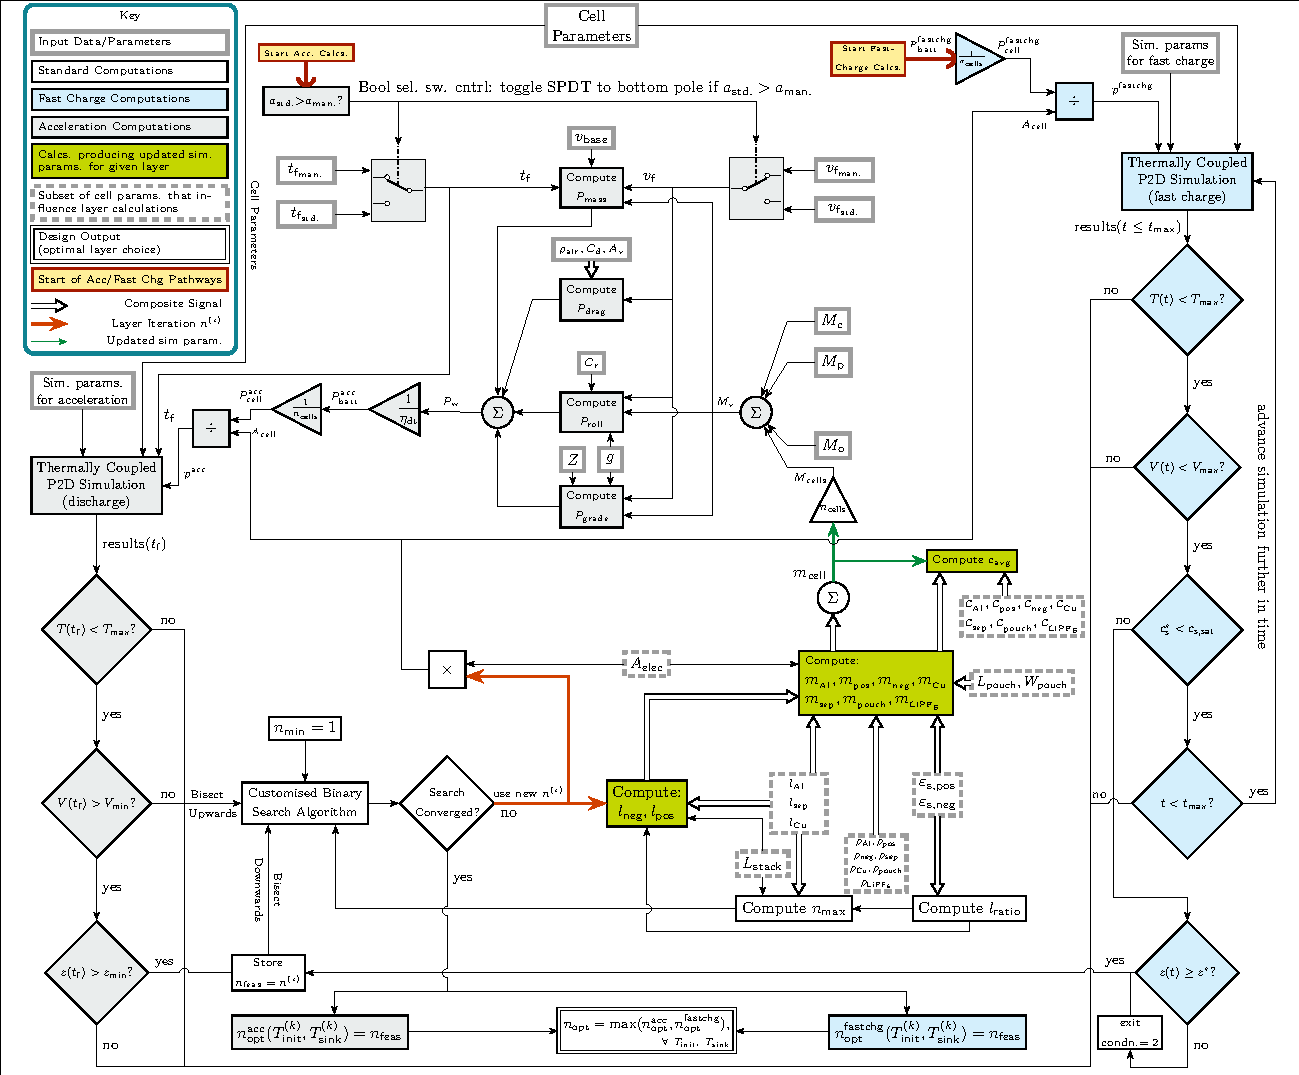
\includegraphics[angle=90, width=\textwidth]{fig_master_flow_diagram}
        \captionsetup{labelsep=note}
        \caption
        [%
        Flow diagram of layer optimisation methodology
        ]%
        {%
            Flow diagram depicting an overview of the proposed layer optimisation methodology
            for Li-ion pouch cells.
        }%
        \label{fig:fig_strategy_schematic}
        \mpfootnotes[1]
        % \vspace*{1.125cm}
        \vspace*{0.7225cm}
        \footnote{This figure was created by \mbox{Krishnakumar Gopalakrishnan} who
            asserts copyright, with intellectual contributions from and the right to
        use asserted by \mbox{Ian D.\ Campbell}.}
    \end{minipage}
\end{figure}

As indicated by  the legend in \cref{fig:fig_strategy_schematic},  blocks with a
light~grey border represent input  data/parameters for computations. Blocks with
a standard black  border represent computations common to  both acceleration and
fast charging pathways. The design output  is given by the double-bordered block
at  the  bottom  centre  of \cref{fig:fig_strategy_schematic}.  Other  types  of
blocks  and arrows  are  appropriately listed  in  the legend  key.  To aid  the
understanding of the  layer optimisation framework, the reader  is encouraged to
correlate  the narrative  in this  section  with the  blocks and  arrows in  the
schematic.  The  acceleration  and  fast  charging  pathways  are  not  amenable
for  standalone comprehension  and  are to  be parsed  in  conjunction with  the
flow  of  control through  the  infrastructure  blocks  as  if the  entire  flow
diagram  is a  single  cohesive unit.  These `control'  blocks,  common to  both
pathways  in \cref{fig:fig_strategy_schematic},  govern how  these two  pathways
are  to be  traversed  with the  presently trialled  layer  choice and  quantify
the  suitable  reformulations needed  whenever  a  new  layer  choice is  to  be
used.  The  computational aspects  covered  by  these  blocks are  described  in
\crefrange{sec:searchalgo}{sec:spheat}.

\subsection{Acceleration pathway}\label{sec:accpathway}

The computations for acceleration-based layer  optimisation begins at the anchor
block labelled `Start Acc.\ Calcs.'.

\subsubsection*{Determination of acceleration rate, final speed and acceleration time}

The  first  step is  to  determine  the rate  of  acceleration  to be  used  for
computing the power requirements for  accelerating an \gls{xeV} from standstill.
For  various  other  regulatory  reasons, vehicular  standards  for  electrified
transport are  codified by various  standardisation bodies (\eg~the SAE~J1772
standard~\cite{Sae2010}). The  standards published by these  regulatory agencies
typically specify  a minimum  required acceleration rate  for the  vehicle under
consideration  to be  certified as  an electric  vehicle. Additionally,  vehicle
manufacturers  often provide  their own  specifications, which  typically exceed
these minimum standards. However, for  certain classes of electric vehicles such
as golf carts,  the manufacturer-specified standards might fall below  that of a
roadworthy  electric vehicle.  This thesis  advocates a  conservative design  by
choosing the higher of the two values.

The  acceleration  rate  is  calculated   by  dividing  a  pre-determined  final
speed~$v_\text{f}$  by the  time~$t_\text{f}$ taken  to attain  that speed  from
standstill.  The  manufacturer-specified  acceleration  rate~$a_\text{man.}$  is
compared  against  the minimum  acceleration  rate  specified by  the  governing
vehicular   standards~$a_\text{std.}$.  The   two  \gls{spdt}   switches  assign
the  final  speed~$v_\text{f}$  and  acceleration  time~$t_\text{f}$  using  the
corresponding values from  the appropriate source depending on which  of the two
acceleration rates is higher.

\subsubsection*{Computation of acceleration power at the wheels}

The  next  step  is  to  calculate   the  acceleration  power  required  at  the
driving wheels~$P_\text{w}$.  Using the  governing equations from  basic vehicle
dynamics (See Maksimovic~\cite{Maksimovic2012}), the power at the wheels of an \gls{xeV} is given
by \cref{eq:wheelpower}.
\begingroup
\allowdisplaybreaks
\begin{subequations}\label{eq:wheelpower}
    \begin{align}
        % \SwapAboveDisplaySkip
        P_\text{w}     & = P_\text{mass} + P_\text{drag} + P_\text{roll} + P_\text{grade} \tag{\ref*{eq:wheelpower}}                  \\
        P_\text{mass}  & = \frac{1}{2} \frac{M_\text{v}(n)}{t_\text{f}} \left(v_\text{b}^2 + v_\text{f}^2\right) \label{eq:masspower} \\
        P_\text{drag}  & = \frac{1}{2} \left(\rho_\text{air} C_\text{d} A_\text{v}v_\text{f}^3\right) \label{eq:dragpower}            \\
        P_\text{roll}  & = C_\text{r} M_\text{v}(n)\, g v_\text{f} \label{eq:rollpower}                                                 \\
        P_\text{grade} & = M_\text{v}(n)\, Z g v_\text{f} \label{eq:gradepower}
    \end{align}
\end{subequations}
\endgroup

The  individual  components  contributing   to  the  summation  for  wheel-power
computation   presented   in    \cref{eq:wheelpower}   is   briefly   explained.
$P_\text{mass}$~represents  the  power  required  to  accelerate  the  vehicle's
mass.   $P_\text{drag}$~and  $P_\text{roll}$~denote   the  powers   required  to
overcome   air  resistance   and  rolling   resistance  respectively.   Finally,
$P_\text{grade}$~represents  the power  required to  negotiate a  road gradient.
Except for $M_\text{v}(n)$  which is described next, all terms  in the \gls{rhs}
of \crefrange{eq:masspower}{eq:gradepower}  are constants. The  nomenclature for
each  of  these  terms   is  explained  in  tables~\ref{tbl:CommonVehicleParams}
and~\ref{tbl:UniqueVehicleParams}  along with  their  numerical  values used  in
simulation.

\subsubsection*{Computation of layer-dependent vehicle mass}\label{sec:layerdependentvehiclemass}

Changing  the layer  count used  within a  cell changes  its mass.  This in-turn
affects the mass of the pack, which further influences the overall vehicle mass.
Hence, for  precise computation  of~$P_\text{mass}$ in  \cref{eq:masspower}, the
vehicle's  mass is  computed  as a  function  of number  of  layers within  each
cell~$n$.

In  the  schematic  of \cref{fig:fig_strategy_schematic},  this  layer-dependent
calculation of  mass of all cells  in the pack~$M_\text{cells}$ is  shown by the
product of  the signal  labelled~$m_\text{cell}$ and  the triangular  gain block
representing the overall number of cells in the pack~$n_\text{cells}$.
\begin{equation}\label{eq:massofallcells}
    M_\text{cells} = n \times m_\text{cell}
\end{equation}

The  mass of  the vehicle  is  given by  the sum  of chassis  mass~$M_\text{c}$,
vehicle payload~$M_\text{p}$, pack overhead~$M_\text{o}$ and the layer-dependent
mass   of   all   cells   in   the  pack~$M_\text{cells}$   as   computed   in
\cref{eq:massofallcells}.   The   computation  of   mass   of   a  single   cell~$m_\text{cell}$ is detailed in \cref{sec:massofonecell}.

\subsubsection*{Computation of acceleration power density per layer}

Since the \gls{p2d} equations of the \gls{dfn} model are based upon a normalised
unit area and is  applicable only to each electrochemical layer,  the goal is to
compute the  power density experienced  by each layer. This  is arrived at  by a
sequence of simple scaling steps.

Firstly, the power demanded  at the pack terminals~$P^\text{acc}_\text{batt}$ is
computed  by  dividing  the  power  at  the wheels  by  the  efficiency  of  the
drivetrain.  As explained  in \cref{subsec:layeroptassumptions},  the drivetrain
consists of  a number  of components,  the efficiencies of  which depend  on the
operating point  (such as the  speed and torque  of the electric  motor, current
drawn  by the  power electronics  etc.). Following  the assumptions  detailed in
\cref{subsec:layeroptassumptions},  a single  lumped efficiency~$\eta_\text{dt}$
can be  used for the powertrain.  The power demand  on the pack is  then divided
by  the  number of  cells  in  the pack~$n_\text{cells}$  to  obtain the  power
demand  at the  input  of the  cell's terminals~$p^\text{acc}_\text{cell}$.  For
each  layer choice~$n$,  the overall  electrochemically active  surface area  is
computed  using by  using \cref{eq:overallarea},  wherein the  surface area  per
layer~$A_\text{elec}$ listed in \cref{tbl:lcoSimParamslayeropt} is held constant
throughout.  Finally, the  acceleration power  density per  layer~$p^\text{acc}$
is  computed  by  dividing  $p^\text{acc}_\text{cell}$ by  the  overall  surface
area~$A_\text{cell}$.

\subsubsection*{Thermally-coupled \glsfmtshort{p2d} simulation and exit
conditions}\label{sec:accexitconditions}

For  the  presently trialled  layer  choice~$n$,  a thermally-coupled  \gls{p2d}
simulation is performed for a duration  of $t_\text{f}$~seconds with the applied
power  density~$p^\text{acc}_\text{cell}$  corresponding  to  the present  layer
choice  as input  to  the  model. When  the  simulation  terminates, the  cell's
condition is compared against three criteria
\begin{enumerate}
    \item the maximum possible values of cell temperature~$T_\text{max}$,
    \item the minimum allowed terminal voltage~$V_\text{min}$, and
    \item the lowest allowed cell \gls{soc}~$z_\text{min}$.
\end{enumerate}
This helps  to determine  whether the  cell constructed  from the  present layer
choice is  able to  successfully satisfy the  acceleration power  demands. These
comparison operations are represented by  decision blocks placed in the leftmost
region of the schematic in \cref{fig:fig_strategy_schematic}.

If  any one  of the  three aforementioned  exit checks  fail, the  present layer
configuration is deemed  to be not feasible and the  entire workflow is repeated
by  trialling a  new  layer  choice. A  sophisticated  search  algorithm, to  be
described  in  \cref{sec:searchalgo}, is  employed  to  minimise the  number  of
iterations  needed  until  a successful  layer  choice~$n_\text{opt}^\text{acc}$
is  obtained.  The above  process  is  repeated  for different  combinations  of
initial and ambient temperatures~${(T_\text{init}, T_\text{sink})}$. The largest
successful  layer value  from  all  temperature combinations  is  deemed as  the
canonical  optimal design  choice  when considering  acceleration demands.  This
concludes the narrative describing the acceleration-specific pathway.


\subsection{Fast-charging pathway}\label{sec:fastchgpathway}

The  workflow describing  the optimal  layer calculation  for the  fast charging
scenario begins  with the  anchor block labelled  `Start Fast-Charge  Calcs.' in
\cref{fig:fig_strategy_schematic}. The charging algorithm used in this framework
is based  upon the model-based strategy  proposed by Choe~\etal~\cite{Choe2013},
wherein  the surface  concentration is  never allowed  to exceed  its saturation
value.  Adopting  this charging  scheme  leads  to  a  robust cell  design  that
is  resilient  to  lithium  plating.  A  major  departure  from  the  scheme  in
Choe~\etal~\cite{Choe2013}  is the  fact that  the constant  current phase  used
therein is replaced  by a constant power  phase. This is so  that the assumption
of  identical  conditions  across  all  cells   in  the  pack  holds  true  (see
\cref{subsec:layeroptassumptions} for  details). Furthermore, the  pulsing phase
used to  top-up the cell's  \gls{soc} in Choe~\etal~\cite{Choe2013}  is omitted.
This  is because,  the level~3  fast charging  specifications typically  require
charging to a  target \gls{soc} that is typically  well below \SI{100}{\percent}
(see \cref{tbl:lcoSimParamslayeropt}).

At     first,     the    charging     power     applied     at    the     pack's
terminals~$P_\text{batt}^\text{fastchg}$ is scaled down by the overall number of
cells in the pack.  This results in the charging power  experienced by each cell
in  the  pack~$P_\text{cell}^\text{fastchg}$.  Following the  strategy  used  in
\cref{sec:accpathway}, the power  at the cell's terminals is scaled  down by the
electrochemically active  overall surface area~$A_\text{cell}$. This  yields the
power density~$p^{\text{fastchg}}$ experienced by each  layer in the cell and is
now  amenable  to be  applied  to  the  normalised  \gls{p2d} equations  of  the
\gls{dfn} model (that has been suitably modified to handle power inputs).

\subsubsection*{Thermally-coupled fast-charging simulations and exit conditions}

After computing  the power  density per  layer, the  thermally-coupled \gls{p2d}
model  is  then  invoked.  While  the  simulation  runs,  the  cell's  state  is
continually evaluated against various termination criteria.
\begin{enumerate}
    \item the maximum possible values of cell temperature~$T_\text{max}$,
    \item the maximum allowed terminal voltage~$V_\text{max}$, and
    \item the surface concentration~$c_\text{s}^{\ast}$ not to exceed the saturation concentration~$c_\text{s,sat}$
\end{enumerate}

If any  of these three criteria  are violated, the simulation  immediately stops
and the trialled layer  choice is deemed to not satisfy  the fast charging power
requirements. The  search algorithm then  updates the layer choice  suitably and
the entire workflow is repeated.

If the  simulation for  any layer choice  passes the  aforementioned termination
criteria,  the  \gls{soc}   achieved  by  the  cell  is   compared  against  the
fast-charging   target~$z^\ast$.  If~${z(t)   >  z^\ast}$,   then  the   present
layer  choice  represents   the  minimum  (and  therefore   optimum)  value  for
this  specific  fast  charging  application.  The  successful  layer  choice  is
labelled~$n_\text{opt}^\text{fastchg}$. If the surface concentration has not yet
reached the saturation limit, then the charge time is compared against the upper
bound for  fast charging specifications~$t_\text{max}$. If  this preset duration
has not been reached, then the simulation is allowed to advance further in time,
with the aforementioned  termination criteria being continuously  tested at each
subsequent time-step.

The above process is repeated for  different combinations of initial and ambient
temperatures~${(T_\text{init},  T_\text{sink})}$.  The  largest  successful
layer value from all temperature combinations is deemed as the canonical optimal
design choice when  considering the fast charging power  demands. This concludes
the  narrative describing  the  fast charging  pathway.

Finally, the  maximum of the  layer choices across all  temperature combinations
from the  acceleration and  fast charging  scenarios is  deemed as  the globally
optimal  number of  layers  to be  used  for this  model-led  cell design. The
maximum value is chosen because, if any smaller layer count is used to construct
the cell, that design shall fail to satisfy its power requirements without
violating at least one termination criterion. Hence, the worst case runs across
all desired thermal scenario under which the cell is intended to operate shall
inform the final design choice.

% Do not forget to quote the value of cs_sat from layer opt paper table and show
% calculation inline. Might even go into the code

\subsection{Search algorithm}\label{sec:searchalgo}

A  customised binary  search algorithm  is designed  for the  layer optimisation
framework.  Binary  search  is  a  computationally  efficient  search  algorithm
requiring a worst-case  operational count of~$\mathcal{O}(\log k)$  where $k$~is
the  overall  number  of  layer  candidates  to  be  searched~\cite{Cormen2009}.
However, this  algorithm is  applicable only  when the array  to be  searched is
already  sorted in  either ascending  or  descending order.  By recognising  the
relationship between the  magnitude of power density applied  versus the factors
that deem a  layer suitable or unsuitable for the  application, a customised set
of `exit conditions'  that meet the aforementioned  sorted-array requirement can
be  enforced. This  specific  mapping is  a  unique  idea and  is  claimed as  a
contribution by this thesis author to the art.

This search  strategy is  equally applicable (with  small modifications  to exit
conditions as explained next) for both acceleration and fast charging pathways.

\subsubsection*{Binary search for acceleration pathway}

If all the termination criteria are  successfully met, the exit condition is set
to a  value of~1. If any  of these conditions  fail, then the exit  condition is
assigned a value of~0. Thus, the search vector in this bespoke strategy consists
of only two Boolean possibilities. For ultra-low layer counts, the applied power
densities are extremely high. Therefore, one of the exit conditions is likely to
fail. For  very high layer  counts, the power  densities are very  low, implying
that acceleration runs shall always be successful. When considering layer counts
from  the lowest  to  the  highest, there  exists  a  critical transition  point
\viz~the  first layer  count  for which  the exit  vector  toggles from~0  to~1.
Through a systematic  bisection of the layer search space,  the search algorithm
speedily converges to the optimal layer value.

\subsubsection*{Binary search for fast-charging pathway}

If all  the fast-charging  termination criteria are  successfully met,  the exit
condition is  set to  a value  of~1. For  violating any  of the  following three
failure conditions (see \cref{sec:fastchgpathway}) \viz~exceeding
\begin{enumerate*}[label=\itshape\alph*\upshape)]
    \item upper cutoff temperature,  or
    \item upper cutoff voltage, or
    \item the maximum allowed charging despite encountering surface saturation,
\end{enumerate*}
the exit condition is  assigned the value of~0. The search  array is bisected by
using  this failed  layer  choice as  the  new lower  bound.  If no  termination
criterion is  violated, then  the presently  trialled layer  choice is  deemed a
success and the exit condition is set to~1. The search space is narrowed down by
using the current layer choice as the new upper bound.

However,  there exists  possible scenarios of needing to assign a  third exit
condition  for the  fast charging case.  If the  aforementioned termination 
criteria  are not  violated, but  the charging process fails to meet  the target
\gls{soc} specification, this implies that the number of layers used is too high
(see \cref{fig:fig_CapacityQuadrants} and \cref{sec:resultslayeropt} for  a
brief explanation of this  case). The exit condition corresponding to this
failure mode is assigned a value of~2. Thus, the search vector in this bespoke
strategy  consists of three distinct numbered exit conditions. Despite being a
failure, from  the perspective of narrowing down the search space,  exit
condition~2 is treated  in the same way  as the  first exit condition \ie~the
trialled layer choice is deemed to be too high.

Akin to the acceleration pathway, the  optimal layer choice for fast charging is
deemed to be at the critical transition point wherein the exit condition toggles
from 0~to~1 and  hence, minimal customisation is needed in  the computer code to
handle these two cases.  The handling of exit condition~2 is  shown in the lower
rightmost portion of \cref{fig:fig_strategy_schematic}. Despite being a failure,
from the search algorithms point of view  this is treated as a success, with the
only difference  being the  assignment of  the exit  condition value  purely for
logging and debugging purposes.

\subsubsection*{Alternative search algorithm --- linear search}

A  simpler alternative  to using  the binary  search algorithm  is the  standard
linear  search  algorithm. This  is  a  simple  search strategy  which  involves
sequentially iterating  from~$n_\text{min}$ to~$n_\text{max}$  until arriving at
the lowest  value~$n_\text{opt}^\text{acc}$  that satisfies all  the termination
criteria. However, a naive use of the linear search algorithm is computationally
expensive with a worst case operation count of~$\mathcal{O}(n)$. Therefore, this
thesis author  recommends the use  of the  bespoke binary search  algorithm. The
choice of minimum and maximum values for  the layer search space is discussed in
\cref{sec:layersearchbounds}.

\subsection{Upper and lower bounds on search space}\label{sec:layersearchbounds}


It is  helpful to determine  the highest possible number  of layers that  can be
physically  accommodated in  a stack  of height~$L_\text{stack}$.  For instance,
this value may be used as the  upper bound to the binary search algorithm (which
compulsorily requires  such an upper bound)  described in \cref{sec:searchalgo}.
This can be obtained by defining a  simple integer optimisation task as shown in
\cref{eq:maxlayersopt}. The objective function here  is to maximise the value of
the layer count~$n$  subject to the physical constraint that  the thicknesses of
both electrodes always remains positive.
\begin{equation}\label{eq:maxlayersopt}
    \begin{aligned}
        \underset{n \, \in \, \mathbb{N}}{\mathbf{max}} \quad & n                                                                                                                                              \\
        \text{s.t.} \quad                                     & l_\text{pos} = \left(\frac{L_\text{stack} - L_\text{Al}(n) - L_\text{Cu}(n) - n l_\text{sep}}{n(1 + l_\text{ratio})}\right) > 0 \\
                                                              & l_\text{neg} = \left(\frac{l_\text{ratio}(L_\text{stack} - L_\text{Al}(n) - L_\text{Cu}(n) - n
l_\text{sep})}{n(1 + l_\text{ratio})}\right) > 0
\end{aligned}
\end{equation}


\Cref{eq:analytical_nmax} represents the analytical  closed-form solution to the
integer optimisation problem of \cref{eq:maxlayersopt}.
\begin{equation}
    \label{eq:analytical_nmax}
    n_\text{max} = \max \left(\floor*{\frac{2\left(L_\text{stack} - l_\text{Cu}\right)}{l_\text{Al}+l_\text{Cu}+2 l_\text{sep}}}, \floor*{\frac{2L_\text{stack} - l_\text{Al} - l_\text{Cu}}{l_\text{Al} + l_\text{Cu} + 2l_\text{sep}}} \right)
\end{equation}

The  first   argument  to  the  $\max$~function  in  \cref{eq:analytical_nmax}
represents the maximum number of physically feasible odd layers while the second
argument  represents  the  maximum  such  value  when  considering  odd  layers.
Therefore, the greater of these two  values is chosen as the maximum permissible
layer choice~$n_\text{max}$ and is used as an input to the search algorithm.


In  the absence  of published  information on  how the  minimum layers  within a
pouch  cell is  currently set,  there is  presently no  unique way  to determine~$n_\text{min}$.  Therefore, for  this  layer optimisation  study,  the value  of
$n_\text{min}$ used  by the  search algorithm  is currently set  to one  --- the
minimum physically feasible number of layers. Design engineers from industry may
opt  to tweak  this to  a higher  value based  on insights  gained from  present
empirical designs.


% \subsubsection*{\hypertarget{href:layerdependentcellmass}{Computation of layer-dependent cell mass}}\label{sec:massofonecell}

\subsection{Electrode thickness ratio for capacity balancing}\label{sec:electroderatio}

A key idea of the layer optimisation  scheme is that, for computing the physical
lengths of  electrodes as a  function of number of  layers, the ratios  of their
thicknesses~$l_\text{ratio}$, is  held constant. This coefficient  is germane to
the concept  of capacity balancing of  electrodes with a view  to equalise their
loading. The  idea of matching  the capacity of  anode and cathode  materials is
widely accepted  as a standard principle  in cell design~\cite{Ramadesigan2012}.
The computation of this $l_\text{ratio}$ parameter is discussed here.

Equating  the active material volume of both electrodes,
\begin{equation}
    A_\text{elec,pos}l_\text{pos}  \varepsilon_\text{s,pos} = A_\text{elec,neg}l_\text{neg}  \varepsilon_\text{s,neg} \label{eq:electrodeCapacity}
\end{equation}

While  stacking the  layers  within a  pouch cell,  for  the negative  electrode
layers, there exists  an extra overhang of~${(<~\SI{2}{mm})}$ with  respect to the
positive  electrode layers.  \Cref{fig:anodeoverhangpouchcell}  shows a  CT~scan
depicting the two-dimensional longitudinal-sections with a close-up view of this
overhang region. This is a design feature  and helps to avoid plating of lithium
at the edges.

\begin{figure}[!htbp]
    \centering
    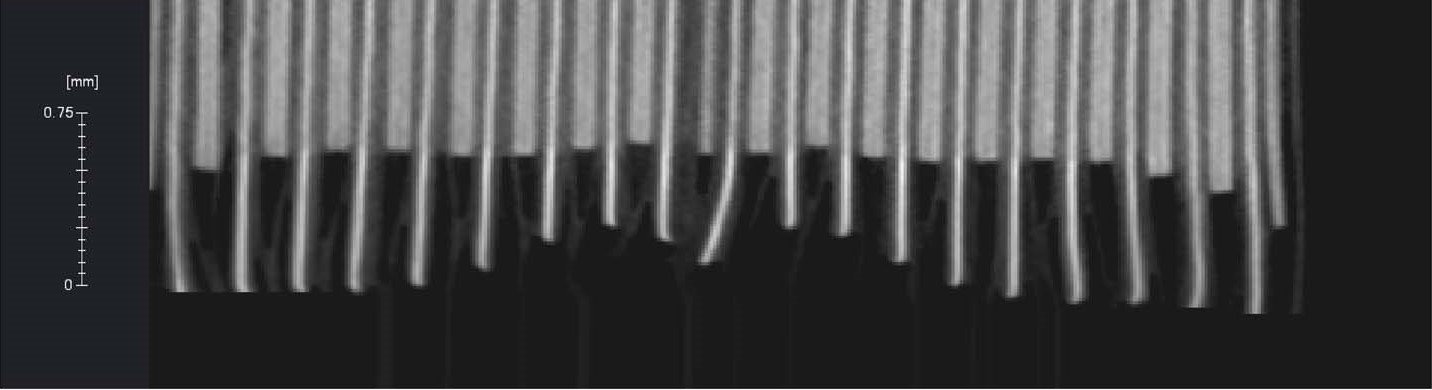
\includegraphics{overhang}
    \caption[Stacking of layers within a pouch cell showing overhang of negative
    electrode]
    {CT~scan showing the two-dimensional longitudinal-sections from the edge of
        the pouch cell with a close-up view of the graphite overhang region. For
        the negative electrode layers, there is an extra overhang of~${(<~\SI{2}{mm})}$ with respect to the positive electrode layers. This
        design feature helps to avoid plating of lithium at the edges. Image
    reproduced from Bond~\etal~\cite{Bond2017}.}
    \label{fig:anodeoverhangpouchcell}
\end{figure}

Neglecting   overhangs    of   the    negative   electrode    (typically   below
$\SI{2}{\milli\meter}$    to    avoid    plating    at    the    edges),    both
electrodes  have  the   same  cross-sectional  area~$A_\text{elec}$.  Therefore,
\cref{eq:electrodeCapacity} reduces to
\begin{align}
    \cancel{A_\text{elec}}l_\text{pos}  \varepsilon_\text{s,pos} & = \cancel{A_\text{elec}}l_\text{neg}  \varepsilon_\text{s,neg}  \\
    l_\text{pos}  \varepsilon_\text{s,pos}                       & = l_\text{neg}  \varepsilon_\text{s,neg}\label{eq:electrodeCapequalarea}
\end{align}

% For    the     reference    cell     under    consideration,     the    length
% and    breadth    of    the    cell's   pouch    is    obtained    from    the
% \gls{bev}    manufacturer~\cite{GMBoltBatteryDims}   and    are   listed    in
% \cref{tbl:lcoSimParamslayeropt}.

Owing to  the reasons outlined in  \cref{subsec:layeroptassumptions}, the volume
fractions  of  the  electrode  materials  are  assumed  to  be  constant,  which
implies  that  their   ratio  is  also  a  constant.   The  electrode  thickness
ratio~$l_\text{ratio}$ is therefore obtained as
\begin{alignat}{2}
    l_\text{ratio} & = \frac{l_\text{neg}}{l_\text{pos}}                                                                                  &  & \qquad\text{(by definition)}                                          \\
    {}             & = \frac{\varepsilon_\text{s,pos}}{\varepsilon_\text{s,neg}}                                                          &  & \qquad\text{(rearranging \cref{eq:electrodeCapequalarea})}           \\
    {}             & = \frac{1-\varepsilon_\text{pos} -
\varepsilon_\text{fi,pos}}{1-\varepsilon_\text{neg} - \varepsilon_\text{fi,neg}}
                   &  & \qquad\text{(by definition, see \cref{eq:volumefraccalc})}                                          \\
    {}             & = \frac{1- 0.385 - 0.025}{1 - 0.485 - 0.033}                                                                         &  & \qquad\text{(substituting values from \cref{tbl:lcoSimParamsSPMp2d})} \\
    l_\text{ratio} & = 1.22\label{eq:electrodeThicknessRatio}
\end{alignat}

\subsection{Computation of electrode thicknesses per layer}

In  this section,  a deterministic  way to  compute the  thickness of  electrode
materials is  present. In  the views  of this thesis  author, this  represents a
departure from  the norm wherein electrode  thicknesses are designed on  a trial
and  error basis~\cite{Ramadesigan2012}.  Following  the  assumptions listed  in
\cref{subsec:layeroptassumptions},  the exterior  dimensions  of  the pouch  are
held  constant. Furthermore,  as explained  in \cref{sec:surfareaperlayer},  the
thickness of  the electrochemical stack within  the pouch cell~$L_\text{stack}$,
is also considered to be constant.  Therefore, when the number of layers forming
the stack is varied,  this implies that the only quantities  that may be allowed
to change are the thicknesses of the two electrodes within each layer \ie~higher
the  layer  count, lower  the  electrode  thicknesses  and vice-versa.  In  this
section, this  relationship between the  number of layers~$n$ and  the electrode
thicknesses~$l_j\ (j  \in {\text{neg},\text{pos}})$ is quantified  with the help
of the key $l_\text{ratio}$ parameter obtained in \cref{sec:electroderatio}.

Figure~2 of Northrop~\etal~\cite{Northrop2011}  (suitably adapted and reproduced
in \cref{fig:topologies})  considers two possible configurations  of stacking up
layers within a pouch cell. In the first topology shown in \cref{fig:topology1},
the outermost current collectors are of copper. In the alternative configuration
shown in  \cref{fig:topology2}, a copper  current collector occupies one  end of
the  stack while  an aluminium  current collector  occupies its  other end.  The
formulae derived  here is equally applicable  to both these cases.  Although the
use of aluminium current collectors at both extrema of the stack is not studied,
the approach presented here may be easily extended to this case.

\begin{figure}[!htbp]
    \centering
    \begin{subfigure}[b]{0.725\textwidth}
        %
        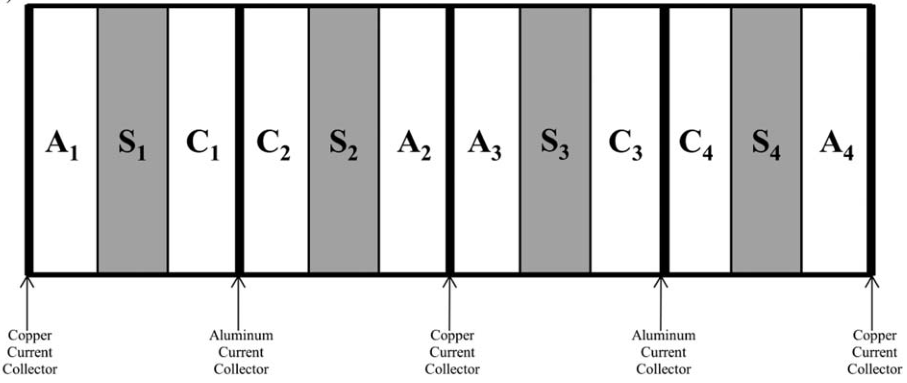
\includegraphics[width=\linewidth]{layer_stack2}
        %
        \caption{Topology 1}
        \label{fig:topology1}
    \end{subfigure}
    \hfill
    \begin{subfigure}[b]{0.225\textwidth}
        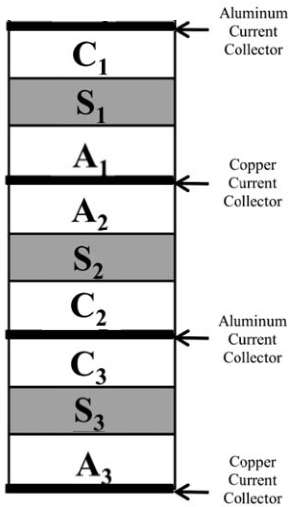
\includegraphics[width=\linewidth]{layer_stack}
        \caption{Topology 2}
        \label{fig:topology2}
    \end{subfigure}
    \caption[Two possible topologies for arranging the layers within a pouch
    cell]
    {Two possible topologies for arranging the layers within a pouch cell. The
        first possibility entails using an even number of layers as shown in the
        example illustration with four layers in the left sub-figure. Here, both
        extrema of the stack are occupied by copper current collectors. The
        second possible arrangement consists of using an odd number of layers
        and  is depicted in the  sample illustration with three layers in
        the right sub-figure. This represents a heterogeneous topology wherein
        the outermost current collectors of the stack consist of copper at one
        end and aluminium at its other end. Illustration adapted from
    Northrop~\etal~\cite{Northrop2011}.}
    \label{fig:topologies}
\end{figure}

The stack height  may be obtained by  the sum of thicknesses  of the constituent
regions.
\begin{align}
    L_\text{stack} &= \sum_jL_j(n) + L_\text{Al}(n) + L_\text{Cu}(n) \qquad\forall \ n \in \mathbb{N},\ j \in \{\text{pos, sep, neg}\} \label{eq:stackThickness}\\
    \shortintertext{where}
    L_j(n) &= n l_j\tag{\ref{eq:stackThickness}a}\\
    L_\text{Al}(n) &=
    \begin{cases}
        \left(\frac{n}{2}\right   )   l_\text{Al},& \text{if $n$ is even} \\
        \left(\frac{n+1}{2}\right )   l_\text{Al},& \text{if $n$ is odd}
    \end{cases}\tag{\ref{eq:stackThickness}b}\\
    L_\text{Cu}(n) &= \begin{cases}
        \left(\frac{n+2}{2}\right )  l_ \text{Cu},& \text{if $n$ is even}\\
        \left(\frac{n+1}{2}\right )  l_ \text{Cu},& \text{if $n$ is odd}\\
    \end{cases}\tag{\ref{eq:stackThickness}c}
\end{align}

The combined thickness of the  two electrode regions in each layer~$l_\text{ce}$
can be then obtained by rearranging \cref{eq:stackThickness}
\begin{equation}
    l_\text{ce} = \frac{L_\text{stack} - \ceil*{0.5(n+1)}l_\text{Cu} - \ceil*{0.5n}l_\text{Al}}{n} - l_\text{sep}\label{eq:combinedElectrodeThickness}
\end{equation}

The    individual     electrode    thicknesses    can    then     be    obtained
from   \cref{eq:combinedElectrodeThickness}   by    suitably   substituting   in
$l_\text{ratio}$ and performing simple algebraic manipulations.
\begin{align}
    l_\text{pos} &= \frac{l_\text{ce}}{l_\text{ratio}+1}\label{eq:lpos}\\
    l_\text{neg} &= l_\text{ce} - l_\text{pos}\label{eq:lneg}
\end{align}

The   values   of   the   two  electrode   thicknesses   thus   obtained   using
\Crefrange{eq:lpos}{eq:lneg}  are used  as computational  domain lengths  in the
\gls{p2d} simulations. Therefore,  these thicknesses have to  be recomputed each
time the trialled number of layers~$n$ is updated by the search algorithm.

\subsection{Computation of layer-dependent cell mass}\label{sec:massofonecell}

The mass of the cell varies as a  function of number of layers. This is because,
the thicknesses  of the  two electrodes  within each layer  changes each  time a
different layer choice is used. Following the discussion in
\cref{sec:electroderatio}, for computing masses of the constituent components of
a cell, the anode overhang is neglected. Therefore, the common cross-sectional
area~$A_\text{elec}$ is used for all calculations. For a given layer choice~$n$,
the cell mass is computed as per \cref{eq:cellmass}.
\begin{subequations}\label{eq:cellmass}
    \begin{align}
        m_\mathrm{cell} &= \sum\limits_{j}m_j + m_\mathrm{Al} + m_\mathrm{Cu} + m_\mathrm{LiPF_6} + m_\mathrm{pouch}, \; j \in  \{\text{pos, sep, neg}\}\tag{\ref*{eq:cellmass}}\\
        m_j &=   A_\mathrm{elec}  L_j \varepsilon_j\rho_j\label{eq:mj}\\
        m_\text{Al} &=   A_\mathrm{elec}  L_\text{Al} \rho_\text{Al}\label{eq:Almass}\\
        m_\text{Cu} &=   A_\mathrm{elec}  L_\text{Cu} \rho_\text{Cu}\label{eq:cumass}\\
        m_\mathrm{LiPF_6} &=   A_\mathrm{elec} \biggl(\sum\limits_{j} L_j (1-
        \varepsilon_{\text{fi}_j}-\varepsilon_j)\biggr)\rho_\mathrm{LiPF_6}\label{eq:lipf6mass} \\
            m_\mathrm{pouch} &= 2H_\mathrm{pouch} L_\mathrm{pouch} W_\mathrm{pouch}
            \rho_\mathrm{pouch}\label{eq:pouchmass}
    \end{align}
\end{subequations}

% \Cref{eq:cellmass}   consists   of  both   constant   components   as  well   as
% components   that  vary   with  the   number  of   layers.  For   instance,  the
% mass  of  the  electrolyte~$m_\text{LiPF6}$  as   well  as  that  of  the  pouch
% material~$m_\text{pouch}$ are constants and are computed only once. 

Owing to lack of information on their thickness, the mass of the cell's tabs has
been omitted in \cref{eq:cellmass}. However, upon availability of the relevant
data, this may be easily incorporated through an equation analogous to
\cref{eq:pouchmass}.

\subsection{Computation of layer-dependent cell specific heat}\label{sec:spheat}

A lumped  thermal model of the  cell given by \cref{eq:thermalmodel}  is used to
model  the  thermal  dynamics  of  the  cell.  This  thermal  model  is  coupled
with  the  electrochemical  model  equations  of the  \gls{p2d}  model  for  the
simulations  used to  determine  the optimal  layer  configurations. The  cell's
temperature~$T_\text{cell}(t)$ is also obtained from this lumped thermal model.
\begin{align}
	m_\text{cell} c_\text{avg} \frac{dT_\text{cell}}{dt} &= -h A_\text{tabs} \left( T_\text{cell}(t) - T_\text{sink} \right) + Q_\text{pol} & \label{eq:thermalmodel}\\
	Q_\text{pol} &= A_\text{cell} \cdot \abs{\mkern1mu i \mkern3mu}\cdot \abs{U - V} & \tag{\ref{eq:thermalmodel}a}\\
	U &= U_\text{pos}(\theta_\text{pos})\bigg|_{\mathrlap{x =
	    x_\text{pos/Alcc}}} -
	    U_\text{neg}(\theta_\text{neg})\bigg|_{\mathrlap{x =
	x_\text{neg/Cucc}}} & \tag{\ref{eq:thermalmodel}b}\\
	V &= \phi_\text{s}\Big|_{\mathrlap{x = x_\text{pos/Alcc}}} \qquad - \phi_\text{s}\Big|_{x = x_\text{neg/Cucc}} & \tag{\ref{eq:thermalmodel}c}
\end{align}

The   average   specific   heat   of    the   cell~$c_\text{avg}$   used   in
\cref{eq:thermalmodel} is  a function of  the number of  layers and is  given by
\cref{eq:spheat}.
\begin{equation}\label{eq:spheat}
    c_\mathrm{avg} = \frac{1}{m_\text{cell}} \biggl[\sum_jc_jm_j + c_\text{Al}m_\text{Al} + c_\text{Cu}m_\text{Cu} + c_\mathrm{LiPF_6}m_\mathrm{LiPF_6} + c_\mathrm{pouch}m_\mathrm{pouch}\biggr],\quad j \in \{\text{pos, sep, neg}\}
\end{equation}

The first  three terms in  \cref{eq:spheat} are evaluated  as a function  of the
number of layers~$n$ by substituting the appropriate layer-dependent mass values
computed  in  \crefrange{eq:mj}{eq:cumass}.  The  latter  two  terms  \ie~the
specific heats of the electrolyte material and the pouch are held constant since
their corresponding mass values do not vary with the number of layers used.

This concludes the overall narrative describing the layer optimisation
framework. The results obtained by applying this methodology to a specific
numerical example is presented in \cref{sec:resultslayeropt}.



\section{Results}\label{sec:resultslayeropt}
% -*- root: ../../main.tex -*
%!TEX root = ../../main.tex
% vim:textwidth=80 fo=cqt conceallevel=0


At the outset, it  is worth mentioning that the focus of this  chapter is on the
layer optimisation \emph{methodology}  itself. The results as such  do not stand
alone  outside of  the  modelling  universe with  all  its inherent  assumptions
discussed  thus far.  Presently,  the value  added  by this  work  is its  ready
adaptability to industry through its  modular design. A numerical implementation
in the form of a toolbox
\footnote{As an accompaniment to this chapter, an open-source software toolbox for optimal layer selection in pouch cells, \viz{} \gls{bold} is made available for download from GitHub. \\ \mbox{\href{https://github.com/ImperialCollegeESE/BOLD_Toolbox}{
\includegraphics [width=0.025\textwidth]{github.pdf}}} \url{ https://github.com/ImperialCollegeESE/BOLD_Toolbox}}
is  also  provided which  is  immediately  available  for  download and  use  by
relevant stakeholders. This author recommends  that until the tool matures, cell
manufacturers  substitute  their  own  parameters  and  adjust  other  numerical
coefficients suitably  so that  the toolbox  supplements, rather  than supplants
present empirical  layer designs. Hence,  the results presented in  this section
must be interpreted in the backdrop  of the context within which the methodology
was developed implying that the reader  must consciously strive to interpret all
numerical  values in  \emph{relative} terms  of magnitude.  To aid  this thought
process, this  author chooses  to deliberately limit  the discussion  around the
\emph{absolute} magnitude of numbers presented here.

\subsection{Modelling Platform and Preconditioning}\label{sec:platformlionsimba}

% -*- root: ../../main.tex -*-
%!TEX root = ../../main.tex
% vim:nospell

\begin{table}[!htbp]
    \small
    \caption[%
    System-level simulation conditions \& thermal parameters of  an \glsfmtshort{lco} cell
    ]%
    {%
        Cell   parameters   and   system   conditions  for   a   simulating   an
        \glsfmtshort{lco} cell  with the  \gls{dfn} electrochemical model  and a
        lumped thermal model. The parameters  presented here when augmented with
        the  values  of  the  kinetic, geometric  and  transport  properties  of
        the  cell (from  \cref{tbl:lcoSimParamsSPMp2d}  represents the  complete
        information  required for  all  simulations in  this layer  optimisation
        framework.
    }%
    \label{tbl:lcoSimParamslayeropt}
    \vspace{-2.6229525pt}
    \begin{threeparttable}
        \centering
        \textbf{System Conditions} \\ \smallskip
        \begin{varwidth}[t]{0.48\linewidth}
            \begin{tabular*}{\textwidth}{@{} l @{\extracolsep{\fill}} S[table-format=1.2,table-space-text-pre=\Tnote{a} ,table-align-text-pre=false] @{}}
                \toprule
                \multicolumn{1}{@{}l}{Parameter} \\
                \midrule

                Lower cutoff cell voltage, $V_\text{min}$ (\si{\volt}) & \Tnote{a} 3.50   \\
                Upper cutoff cell voltage, $V_\text{max}$ (\si{\volt}) & \Tnote{b} 4.22   \\

                \bottomrule
            \end{tabular*}
        \end{varwidth}
        \hfill
        \begin{varwidth}[t]{0.48\linewidth}
            \begin{tabular*}{\textwidth}{@{} l @{\extracolsep{\fill}} S[table-format=2.2,table-space-text-pre=\Tnote{a} ,table-align-text-pre=false] @{}}
                \toprule
                \multicolumn{1}{@{}l}{Parameter} \\
                \midrule

                Target cell SOC for fast charge, $z^\ast$ \si{(\%)}                & \Tnote{c} 80.00 \\
                Cell upper temperature limit, $T_\text{max}$ \si{(\degreeCelsius)} & \Tnote{d} 55.00 \\

                \bottomrule
            \end{tabular*}
        \end{varwidth}

        \medskip
        \begin{tabular*}{\textwidth}{@{} l @{\extracolsep{\fill}} r @{}}
            \multicolumn{2}{c}{\textbf{Geometric Parameters}} \\
            \toprule
            \multicolumn{1}{@{}l}{Parameter} \\
            \midrule
            Surface area of pos.\ \& neg.\ electrode overlap within a layer, {$A_\text{elec}$} \si{(m^2)} & \textsuperscript{b}\num{4.19e-2}   \\
            Exterior pouch length, $L_\text{pouch}$ \si{(m)}                                              & \textsuperscript{e}\num{332.74e-3} \\
            Exterior pouch width, $W_\text{pouch}$ \si{(m)}                                               & \textsuperscript{e}\num{99.06e-3}  \\
            Exterior pouch height, $H_\text{pouch}$ \si{(m)}                                              & \textsuperscript{f}\num{10.00e-3}  \\
            Pouch material thickness, $T_\text{pouch}$ \si{(m)}                                           & \textsuperscript{g}\num{160.00e-6} \\
            \bottomrule
        \end{tabular*}
        \medskip
        \centering \textbf{Thermal Parameters} \\ \smallskip
        \resizebox{\textwidth}{!}{%
            \begin{tabular}{@{} l S[table-format=4.0,table-space-text-pre=\Tnote{m} ,table-align-text-pre=false] S[table-format=4.1,table-space-text-pre=\Tnote{m} ,table-align-text-pre=false] S[table-format=4.1,table-space-text-pre=\Tnote{m} ,table-align-text-pre=false] S[table-format=4.2,table-space-text-pre=\Tnote{m} ,table-align-text-pre=false] S[table-format=4.0,table-space-text-pre=\Tnote{m} ,table-align-text-pre=false] S[table-format=4.1,table-space-text-pre=\Tnote{m} ,table-align-text-pre=false] S[table-format=4.1,table-space-text-pre=\Tnote{m} ,table-align-text-pre=false] @{}}
                \toprule
                \multicolumn{1}{@{}l}{Parameter} & \multicolumn{1}{c}{Al.\ CC} & \multicolumn{1}{c}{Pos} & \multicolumn{1}{c}{Sep} & \multicolumn{1}{c}{Neg} & \multicolumn{1}{c}{Cu.\ CC} & \multicolumn{1}{c}{\ch{LiPF_6}} & \multicolumn{1}{r@{}}{Pouch}\\
                \midrule

                Sp.\ heat capacity, $c_j$ (\si{\joule\per\kilogram\per\kelvin})   & \Tnote{h} 903  & \Tnote{h} 1269.2 & \Tnote{h} 1978.2 & \Tnote{h} 1437.4 & \Tnote{h} 385  & \Tnote{h} 2055.1 & \Tnote{i} 1464.8 \\
                Density, $\rho_j$ (\si{\kilogram\per\meter\cubed})                & \Tnote{j} 2700 & \Tnote{k} 2291.6 & \Tnote{b} 1100.0 & \Tnote{j} 2660.0 & \Tnote{l} 8960 & \Tnote{j} 1290.0 & \Tnote{m} 1150.0 \\
                Activ.\ energy, diff. ${E_\text{act,s}}_j$ (\si{\joule\per\mole}) & {---}                   & \Tnote{p} 5000   & {---}                     & \Tnote{p} 5000   & {---}                   & {---}                     & \multicolumn{1}{c}{---}   \\
                Activ.\ energy, rxn. ${E_\text{act,k}}_j$ (\si{\joule\per\mole})  & {---}                   & \Tnote{p} 5000   & {---}                     & \Tnote{p} 5000   & {---}                   & {---}                     & \multicolumn{1}{c}{---}   \\

                \bottomrule
            \end{tabular}
        }
        \medskip
        \begin{tabular*}{\textwidth}{@{} l @{\extracolsep{\fill}} r @{}}
            \multicolumn{2}{c}{\textbf{Other Geometric/Cell-Level Parameters}} \\
            \toprule
            \multicolumn{1}{@{}l}{Parameter} \\
            \midrule

            Thickness of pos.\ current collector, $l_\text{Al}$ \si{(m)}                    & \textsuperscript{f}\num{15e-6}   \\
            Thickness of neg.\ current collector, $l_\text{Cu}$ \si{(m)}                    & \textsuperscript{p}\num{10e-6}   \\
            Total tab area, $A_\text{tabs}$ \si{(m^2)}                                      & \textsuperscript{b}\num{5.94e-3} \\
            Lumped heat transfer coefficient, $h$ (\si{\watt\per\meter\squared\per\kelvin}) & \textsuperscript{b}150           \\
            Initial electrolyte concentration, $c_\text{e,0}$ (\si{\mole\per\meter\cubed})  & \textsuperscript{q}1000          \\

            \bottomrule
        \end{tabular*}

        \medskip
        \begin{tabular*}{\textwidth}{@{} =P{7.5cm}  +l@{\extracolsep{\fill}}+c +r @{}}
            \multicolumn{4}{c}{\textbf{Spatial Discretisation}} \\
            \toprule
            \multicolumn{1}{@{}l}{Parameter} & \multicolumn{1}{l}{Pos} & \multicolumn{1}{c}{Sep} & \multicolumn{1}{r@{}}{Neg}\\
            \midrule

            Nodes, through-thickness (axial), $N_{\text{a}_j}$          & \num{40} & \num{40} & \num{40} \\
            Nodes, within spherical particle (radial), $N_{\text{r}_j}$ & \num{15} & ---      & \num{15} \\

            \bottomrule
        \end{tabular*}

        \medskip
        \vspace{-2.6229525pt}
        \begin{tablenotes}[para,flushleft]
            \begin{footnotesize}
            \item[a] Calculated as described in \cref{sec:cutoff}
            \item[b] Assumed
            \item[c] Ref.~\cite{Sae2010}
            \item[d] Ref.~\cite{Kizilel2009} \\
            \item[e] Converted from imperial units reported in~Ref.~\cite{GMBoltBatteryDims}
		    \item[f] Table~\romanletter{4} of~Ref.~\cite{Groger2015} \\
            \item[g] Sum of values in table~1 of~Ref.~\cite{Svens2013}
            \item[h] Ref.~\cite{Chen2005}
            \item[i] Computed from values of constituents (see~\cite{Svens2013}) using Ref.~\cite{martienssen2006springer} \\
            \item[j] Ref.~\cite{Guo2010}
            \item[k] Ref.~\cite{Jeon2011}
            \item[l] Ref.~\cite{Worwood2017,Song2000}
            \item[m] Ref.~\cite{Kim2009}
            \item[p] Ref.~\cite{Northrop2011}
            \item[q] Ref.~\cite{Subramanian2009}
            \end{footnotesize}
        \end{tablenotes}
    \end{threeparttable}
\end{table}



The   complete   parameter   set   used   for   simulation   is   presented   in
\cref{tbl:lcoSimParamslayeropt}.  All   cells  are   assumed  to  be   in  their
equilibrium  state prior  to  beginning of  simulations. The  thermally-coupled,
\gls{p2d}  electrochemical  model  used  for simulating  each  layer  choice  is
implemented  in MATLAB~\cite{matlab}  using  a heavily-modified  version of  the
LIONSIMBA toolbox~\cite{Torchio2016}.  The work reported in  this chapter helped
to advance the  toolbox from~v1.0x to~v2.0. The updated computer  codes to which
this author heavily contributed,
is available from the project's official repository\footnote{LIONSIMBA~v2:
\mbox{\href{https://github.com/lionsimbatoolbox/LIONSIMBA}{
\includegraphics
[width=0.025\textwidth]{github.pdf}}} \url{
https://github.com/lionsimbatoolbox/LIONSIMBA}}.

The  rationale  behind  choosing  this  specific  software  to  implement  layer
optimisation  is  as  follows.  The LIONSIMBA~v1.0x  toolbox  has  already  been
validated against  the results of the  DUALFOIL~\cite{Dualfoil1998} codes (which
can be considered as the present benchmark standard). The toolbox is implemented
in the  MATLAB programming language.  Since this  chapter has a  strong industry
focus,  the  omnipresence  of  MATLAB  in industry,  its  mature  code-base  and
familiarity  was  a strong  motivator  in  the  adoption  of this  toolbox.  The
simulation  speeds using  LIONSIMBA  have been  shown to  be  comparable to  the
FORTRAN  implementation  of  DUALFOIL,  primarily  owing  to  the  sophisticated
computation  of  the  analytical  Jacobian   of  the  system  through  automatic
differentiation~\cite{Torchio2016}.  In  addition  to  fundamental  enhancements
to  the   modelling  platform  presented   in  \cref{sec:numericalenhancements},
numerous  bug fixes  and  other  minor enhancements  to  the original  LIONSIMBA
code-base  have  been  provided  by   this  thesis  author.  Interested  readers
may  peruse   these  from  the   \texttt{README.md}  file  from   the  project's
\href{https://github.com/lionsimbatoolbox/LIONSIMBA}{repository}.

\subsection{\glsfmtshort{xeV} configurations}

% -*- root: ../../main.tex -*-
%!TEX root = ../../main.tex
% vim:nospell


\begin{table}[!htbp]
	\renewcommand{\thetable}{\arabic{table}a}
	\centering
	\caption{Acceleration test parameters (common across xEV platforms)}
	\label{tbl:CommonVehicleParams}
	\sisetup{table-format=3.2, table-number-alignment=center, table-space-text-pre=\textsuperscript{a}, table-space-text-post=\textsuperscript{a}, table-align-text-post=false}
	\begin{threeparttable}[t]
		\centering
		\begin{tabular}{@{} l  S @{}}
			\toprule
			Parameter \\
			\midrule

			% Coefficient of drag for xEV body, $C_\mathrm{d}$                           & {\makebox*{00}[r]{\tnote{a}}} 0.31                \\
			% Frontal area of xEV, $A_\mathrm{v}$ \si{(m^2)}                             & {\makebox*{00}[r]{\tnote{b}}} 2.40                \\
			% Acc.\ time specified by manufacturer, $t_\mathrm{f,man}$ \si{(s)}          & {\makebox*{00}[r]{\tnote{d}}} 6.50                \\
			% Acc.\ time dictated by standards, $t_\mathrm{f,std}$ \si{(s)}              & {\makebox*{00}[r]{\tnote{c}}} 6.00                \\
			% Speed, end of acc. (standards), $v_\mathrm{f,std}$ \si{(m.s^{-1})}         & {\makebox*{00}[r]{\tnote{e}}} 8.94                \\
			% Speed, end of acc. (manufacturer), $v_\mathrm{f,man}$ \si{(m.s^{-1})}      & {\makebox*{0}[r]{\tnote{f}}} 26.82                \\
			% Base speed of  xEV, $v_\mathrm{b}$ \si{(m.s^{-1})}                         & {\makebox*{\hspace*{0.5mm}0}[r]{\tnote{e}}} 13.41 \\
			% Air density at acc.\ test conditions, $\rho_\mathrm{air}$ \si{(kg.m^{-3})} & {\makebox*{\hspace*{0.5mm}00}[r]{\tnote{f}}} 1.20 \\
			% Drivetrain efficiency, $\eta_\mathrm{dt}$                                  & {\makebox*{00}[r]{\tnote{g}}} 0.75                \\
			% Payload, $M_\mathrm{p}$ \si{(kg)}                                          & {\hspace*{0.00005mm}{\tnote{c}}} 150.60 \\
			% Rolling resistance coefficient of road surface, $C_\mathrm{r}$             & {\makebox*{00}[r]{\tnote{f}}} 0.01                \\
			% Road gradient, $Z$                                                         & {\makebox*{00}[r]{\tnote{g}}} 0.00                \\

			Coefficient of drag for xEV body, $C_\mathrm{d}$                           & 0.31   {\tnote{a}} \\
			Frontal area of xEV, $A_\mathrm{v}$ \si{(m^2)}                             & 2.40   {\tnote{b}} \\
			Acc.\ time specified by manufacturer, $t_\mathrm{f,man}$ \si{(s)}          & 6.50   {\tnote{d}} \\
			Acc.\ time dictated by standards, $t_\mathrm{f,std}$ \si{(s)}              & 6.00   {\tnote{c}} \\
			Speed, end of acc. (standards), $v_\mathrm{f,std}$ \si{(m.s^{-1})}         & 8.94   {\tnote{e}} \\
			Speed, end of acc. (manufacturer), $v_\mathrm{f,man}$ \si{(m.s^{-1})}      & 26.82  {\tnote{f}} \\
			Base speed of  xEV, $v_\mathrm{b}$ \si{(m.s^{-1})}                         & 13.41  {\tnote{e}} \\
			Air density at acc.\ test conditions, $\rho_\mathrm{air}$ \si{(kg.m^{-3})} & 1.20   {\tnote{f}} \\
			Drivetrain efficiency, $\eta_\mathrm{dt}$                                  & 0.75   {\tnote{g}} \\
			Payload, $M_\mathrm{p}$ \si{(kg)}                                          & 150.60 {\tnote{c}} \\
			Rolling resistance coefficient of road surface, $C_\mathrm{r}$             & 0.01   {\tnote{f}} \\
			Road gradient, $Z$                                                         & 0.00   {\tnote{g}} \\

			\bottomrule
		\end{tabular}
        \begin{tablenotes}[para,flushleft]
        \item[a]Ref.~\cite{HybridCars2017Drag}
        \item[b]Calculated from typical \gls{bev} dimensions in~\cite{BoltDimensions}
        \item[c]Ref.~\cite{ETANTP002-2004}
        \item[d]Ref.~\cite{BoltOverview}
        \item[e]Ref.~\cite{Liu2016a}
        \item[f]Ref.~\cite{EmadiElectric}
        \item[g]Assumed
        \end{tablenotes}
	\end{threeparttable}
\end{table}


Tables~\ref{tbl:CommonVehicleParams} and~\ref{tbl:UniqueVehicleParams}  show the
\gls{xeV}  parameters used  in simulations.  The  power demands  on the  battery
pack  during  normal  operation  are   found  to  be  significantly  lower  than
that  experienced during  the  two  extreme cases  of  discharging and  charging
\viz{} \emph{acceleration} and \emph{fast  charging} respectively. For instance,
\SI{50.83}{\kilo\watt} is the peak  discharge power while \SI{14.20}{\kilo\watt}
is  the median  discharge power  for various  standard drive  cycles. Even  with
the  assumption that  \SI{100}{\percent}  of braking  energy  can be  recovered,
the  peak  and  median  charging  powers  are  only  \SI{43.13}{\kilo\watt}  and
\SI{26.03}{\kilo\watt}  respectively.

The   discharging  and   charging  powers   experienced  by   the  pack   during
acceleration and  fast charge  are significantly  higher than  those experienced
with  any  standard  drivecycle.  Considering  the  acceleration  parameters  in
\cref{tbl:CommonVehicleParams} for  the \gls{bev}  pack, \SI{181.45}{\kilo\watt}
is   the  power   requirement  for   acceleration  of   a  fixed   vehicle  mass
on   a   flat  road   surface.   Four   distinct  fast-charging   power   levels
\viz{}   \SI{50}{\kilo\watt},   \SI{80}{\kilo\watt},  \SI{110}{\kilo\watt}   and
\SI{130}{\kilo\watt}  are considered  in this  study.  This is  in adherence  to
the  minimum  and maximum  values  of  level~3  rating  as suggested  by  Yilmaz
and~Krein~\cite{Yilmaz2012}. Furthermore, near-term fast charging goals laid out
in  literature~\cite{Ashique2017,Srdic2016} and  the  peak  power capability  of
charging infrastructure further justify these choices.

% -*- root: ../../main.tex -*-
%!TEX root = ../../main.tex
% vim:nospell


\begin{table}[!htbp] % Parameters unique to each of the BEV & PHEV
	% \addtocounter{table}{-1}
	% \renewcommand{\thetable}{\arabic{table}b}
	\caption{Acceleration test parameters (specific to each \glsfmtshort{xeV})}
	\label{tbl:UniqueVehicleParams}
	\centering
    \sisetup{table-format=4.1, table-number-alignment=center, table-space-text-pre=\textsuperscript{a}, table-align-text-pre=false}
	\begin{threeparttable}[t]
		\begin{tabular*}{0.72\textwidth}{@{} l @{\extracolsep{\fill}}  S S @{}}	% Works with Tnote
			\toprule
			\multicolumn{1}{@{} l}{Parameter} & \multicolumn{1}{c}{BEV} & \multicolumn{1}{c@{}}{PHEV} \\
			\midrule

			Mass of xEV chassis, $M_\mathrm{c}$ \si{(kg)}               & \Tnote{a} 1340.0 & \Tnote{b} 1438.0 \\
			Mass of pack overhead (w/o cells), $M_\mathrm{o}$ \si{(kg)} & \Tnote{a} 196.4  & \Tnote{c} 65.5   \\
			Upper cutoff SOC of cell, $z_\mathrm{max}$ \si{(\%)}        & \Tnote{d} 95.0   & \Tnote{d} 90.0   \\
			Lower cutoff SOC of cell, $z_\mathrm{min}$ \si{(\%)}        & \Tnote{d} 5.0    & \Tnote{e} 30.0   \\

			\bottomrule
		\end{tabular*}
		\begin{tablenotes}[para,flushleft]
		\item[a]Calculated based on~\cite{ChevyBoltSpecs}
		\item[b]Calculated based on~\cite{motortrendEcotec,ChevyBoltSpecs}
		\item[c]Calculated (see sections~\ref{sec:layerdependentvehiclemass} \& \ref{sec:massofonecell})
		\item[d]Assumed
		\item[e]Ref.~\cite{EmadiElectric}
		\end{tablenotes}

	\end{threeparttable}
\end{table}


For  the  acceleration  tests,  the  initial cell  \gls{soc}  has  been  set  to
\SI{40}{\percent}.  This  is  in  conformity with  the  test  criterion  $(50\pm
10)$~\%  of  the  SAE~J1666   standard~\cite{Sae2010}.  By  choosing  the  worst
case  starting  \gls{soc} \ie{}  \SI{40}{\percent},  a  conservative design  can
be  achieved.  The  chassis  mass  of  the  vehicle  as  well  as  the  mass  of
two  passengers   at  75.3  kg   each~\cite{Sae2010}  is  considered   for  both
\gls{xeV}  platforms. The  pack mass  is  computed as  a function  of number  of
layers  as  described  in  \cref{sec:layeroptframework}.  Vehicle  manufacturers
General  Motors  Inc.\, provide  the  mass  value of  the  GM  Ecotec series  of
engines~\cite{motortrendEcotec} that can  be used for the  \gls{phev} case which
consists of  a range-extending \gls{ice}.  The mass  of the Bolt  \gls{bev} pack
reported in~\cite{ChevyBoltSpecs} minus  the computed mass of  the overall cells
used in the pack  gives the overhead mass of the  \gls{bev} pack. The \gls{phev}
pack's  overhead  mass  is  determined  by suitably  scaling  the  mass  by  the
proportion of reduction in the number of cells used.


For the \gls{bev}  platform, a fast-charging scheme operated on  a \gls{cp} mode
with an initial  \gls{soc} of \SI{20}{\percent} is employed. In  the case of the
\gls{phev}, an initial \gls{soc}  of \SI{30}{\percent} (\SI{10}{\percent} higher
than that for \gls{bev}) is used. This facilitates a smaller \gls{soc} window by
taking  into account  the higher  number  of charge-discharge  cycles which  are
typical with \gls{phev}  designs~\cite{Maksimovic2012}. Both \gls{xeV} platforms
are fast  charged to a target  \gls{soc} of \SI{80}{\percent} in  \gls{cp} mode.
This \gls{soc} value corresponds to the end-of-charge target in level~3 charging
standards~\cite{SAECharging2011}.

\subsection{Acceleration studies}

For both vehicle platforms under study, the acceleration at a worst-case rate of
\SI{4.13}{\meter\per\second\squared} is assumed for simulation. This corresponds
to the  manufacturer's acceleration specifications  for the \gls{bev}  listed in
\cref{tbl:CommonVehicleParams}.  The  acceleration  rate  corresponding  to  the
SAE~J1772 standards is lower than this  rate. Therefore, to obtain a robust cell
design, the higher of the two acceleration rates needs to be considered.

\Cref{tbl:accResults}  gives the  simulation  results  for various  combinations
of  $(T_\text{init},  T_\text{sink})$  for  both the  \gls{bev}  and  \gls{phev}
platforms. The following discussion is applicable for both vehicular platforms.

% -*- root: ../../main.tex -*-
%!TEX root = ../../main.tex
% vim:nospell

\begin{table}[htb!]
    \caption{\glsfmtshort{xeV} acceleration test results}
    \label{tbl:accResults}
    \centering
	\begin{tabular}{c c c}
        \toprule
        \multicolumn{1}{@{} l}{\makecell{($T_\text{init},T_\text{sink}$) \\ \footnotesize (degC)}} & \makecell{$n^\text{acc}_\text{opt}$ \\ \footnotesize \glsfmtshort{bev}}&  \multicolumn{1}{c @{}}{\makecell{$n^\text{acc}_\text{opt}$ \\ \footnotesize \gls{phev}}}  \\
        \midrule

        (38,5)  & \num{21} & \num{55} \\
        (38,49) & \num{21} & \num{57} \\
        (25,25) & \num{23} & \num{63} \\
        (15,5)  & \num{27} & \num{69} \\

        \bottomrule
    \end{tabular}
\end{table}


The  specific combinations  of temperatures  for traversing  the thermal  design
space are  chosen following the  SAE~J1772 guidelines. The high  power densities
resulting from  low numbers of layers  lead to large overpotentials  causing the
cell's terminal  voltage to  drop lower than  $V_\text{min}$, thereby  unable to
satisfy acceleration requirements. However,  at higher $T_\text{init}$, owing to
the  reduction in  overpotentials, a  larger  voltage overhead  is available  to
accommodate the  internal polarisation  drop. For all  temperature combinations,
the largest deviation from $T_\text{init}$  experienced by the \gls{bev} cell is
a \SI{0.48}{\degreeCelsius} increase.  Consequently, it can be  concluded that a
single isolated acceleration event does not heat the \gls{bev} battery pack, and
therefore the cell  temperature remains close to that of  the initial value. The
\gls{phev} cell  experiences higher  power levels  and although  its temperature
increases  much  higher  than  the corresponding  \gls{bev}  cell,  the  maximum
temperature  during acceleration  remains  well below  the  upper cutoff  limit.
Furthermore, even  for the worst  case simulation  run, the cell's  \gls{soc} is
depleted only by  a maximum value of \SI{0.32}{\percent} for  the \gls{bev} cell
and by a slightly higher value for the \gls{phev} cell.

The foregoing  discussion has revealed  that the lower cut-off  voltage strongly
influences  layer   configuration  for   acceleration  tests.   Therefore,  when
considering acceleration requirements, $n = 27$ and $n=69$ represent the optimal
layer choices for the \gls{bev} and \gls{phev} platforms respectively .

\subsection{Fast-charging studies}

\begin{figure}[p]
    \begin{minipage}[t]{\textwidth}
        \centering
        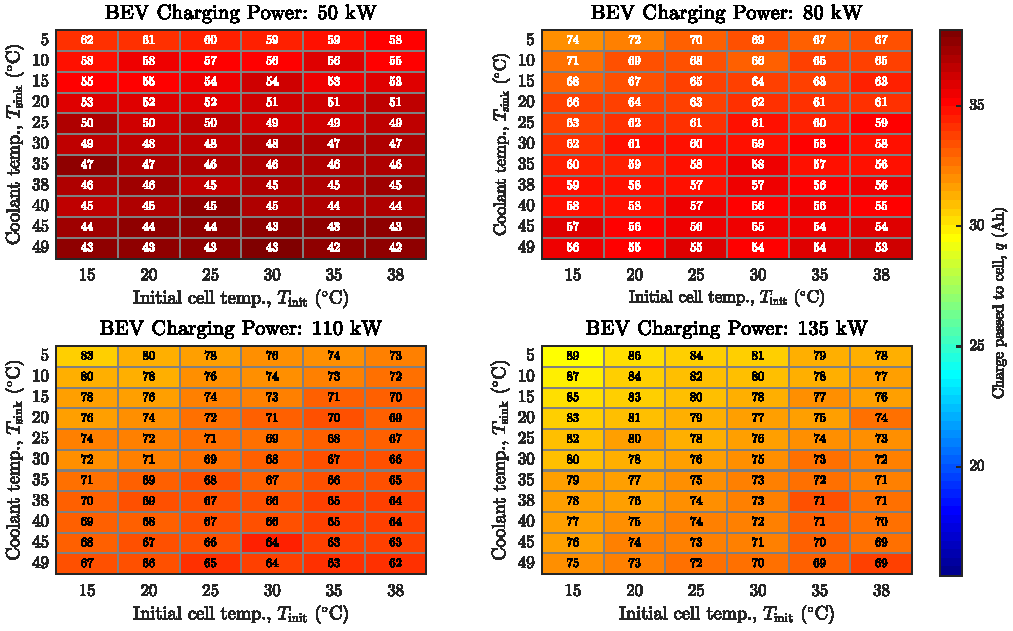
\includegraphics[width=\textwidth]{fig_generate_heatmap_BEV}
        \captionsetup{labelsep=note}
        \caption[Optimal cell layer configurations for the \gls{bev}, presented for a range of fast charging powers and thermal conditions]{Optimal cell layer configurations for the \gls{bev}}
        \label{fig:fig_generate_heatmap_BEV}
        \setcounter{footnote}{8}
        \vspace*{\floatsep}
        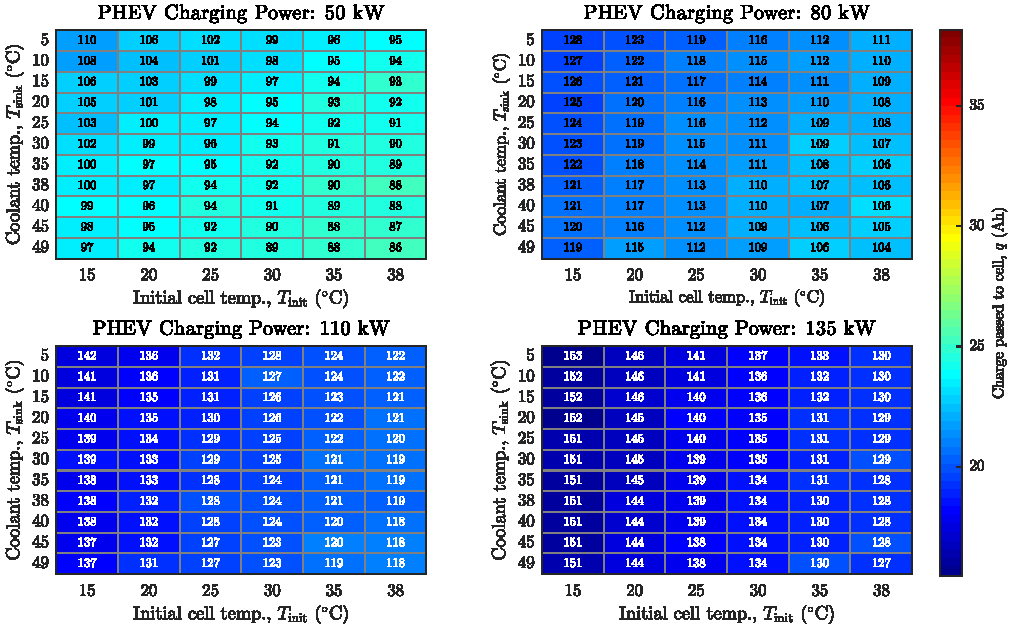
\includegraphics[width=\textwidth]{fig_generate_heatmap_PHEV}
        \caption[Optimal cell layer configurations for the \gls{phev}, presented for a range of
        fast charging powers and thermal conditions]{Optimal cell layer configurations for the \gls{phev}}
        \label{fig:fig_generate_heatmap_PHEV}
        \mpfootnotes[1]
        \footnote{These figures were created by \mbox{Ian D.\ Campbell} who asserts copyright,
            with intellectual contributions from and the right to use asserted by
        \mbox{Krishnakumar Gopalakrishnan}.}
    \end{minipage}
\end{figure}

Figures~\ref{fig:fig_generate_heatmap_BEV}
and~\ref{fig:fig_generate_heatmap_PHEV} shows the results  produced by the layer
optimisation framework  for the \gls{bev} and  \gls{phev} platforms respectively
when  considering fast  charging requirements.  Each heat~map  in these  figures
show  the optimal  number  of  layers~$n^\text{fastchg}_\text{opt}$ for  various
combinations of  initial and  ambient temperatures  for four  different charging
powers. In each case, the  values of $n^\text{fastchg}_\text{opt}$ correspond to
the  temperature  combination  \mbox{$(T_\text{init},T_\text{sink})  =  (15,  5)
\si{\degreeCelsius}$}  as  shown  in  \cref{fig:fig_generate_heatmap_BEV}.  This
represents the  least number of  layers required to  fast charge the  pack under
\gls{cp} conditions until  the target \gls{soc} is reached.  The charging scheme
additionally considers the constraint that the cell temperature must stay within
\mbox{$T_\text{max}=  \SI{55}{\degreeCelsius}$}. Furthermore,  its voltage  must
remain less than or equal  to \mbox{$V_\text{max} = \SI{4.22}{\volt}$}. Finally,
the charging algorithm is plating-aware \ie{}  the charging stops as soon as the
concentration at the particle surface reaches the maximum possible concentration
limit, thereby preventing  lithium plating at the surface  of negative electrode
particles.


Thus,   using    the   model-based    design   strategy   presented    in   this
chapter,   an   effective    cell   design   is   achieved    which   helps   to
maximise   energy   density  and   \gls{bev}   range,   without  forgoing   fast
charging   power    targets.   From   figures~\ref{fig:fig_generate_heatmap_BEV}
and~\ref{fig:fig_generate_heatmap_PHEV},       it       is       seen       that
$n^\text{fastchg}_\text{opt}$  increases with  increase in  the charging  power.
This is because,  as the charging power increases, the  minimum number of layers
required to maintain  the cell voltage below the maximum  permissible value also
increases.  This requires  higher interfacial  surface area  to accommodate  the
increased  power demand.  Furthermore, rapid  surface saturation  occurs due  to
steep  concentration  profiles in  the  negative  electrode particles  when  the
charging power is  high which causes plating. With higher  layers, the resulting
electrodes  are thinner,  thereby allowing  faster diffusion  of lithium  in the
solid  particles  and  avoiding  steep concentration  gradients  in  them.  This
suggests that the number of layers must be large enough to prevent plating.

\Cref{fig:fig_CapacityQuadrants} shows the nominal  capacity of cells and charge
passed versus  the number of  layers during fast  charging. In these  plots, the
theoretical  capacity~$Q_\text{n}$ of  the cell  versus the  layer count~$n$  is
represented by the linear downward-sloping line.

\begin{figure}[!bp]
    \begin{minipage}[t]{\textwidth}
        \centering
        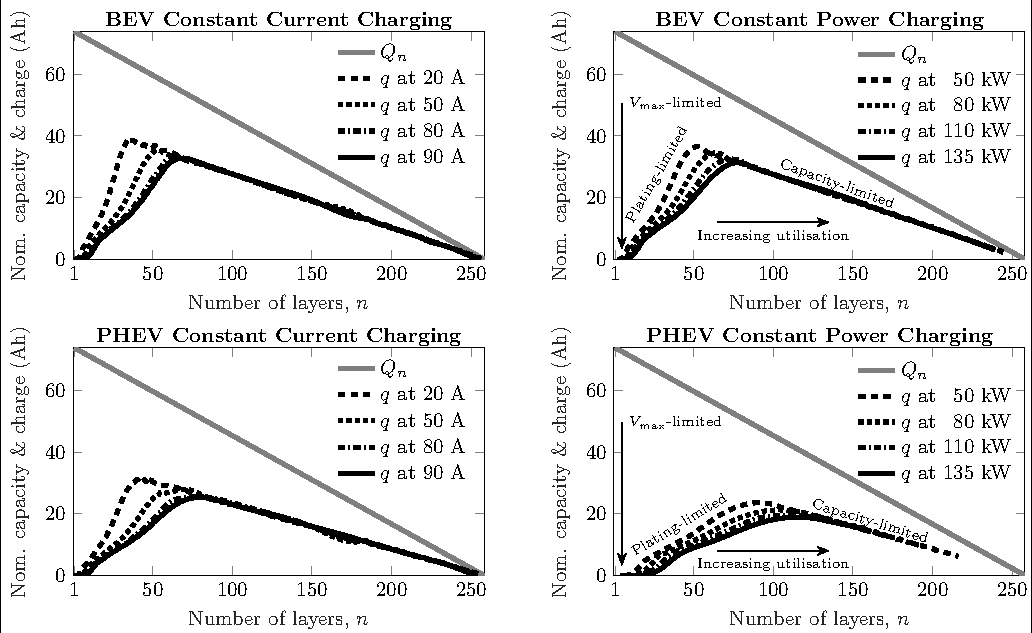
\includegraphics[width=0.998046875\textwidth,trim=4 2 3 4,clip]{fig_capacity_quadrants.pdf}
        \captionsetup{labelsep=note}
        \caption[
        Nominal capacity and charge passed versus layer count for ---
        \emph{a}) constant current  charging and \emph{b}) constant power  charging
        ]
        {
            The right column shows nominal cell capacity and charge passed
            during \gls{cp} charging. Rate capability and cell utilisation are positively
            correlated with $n$. With increasing power levels, the optimal layer configuration shifts to higher
            values of $n$. Similar behaviour is observed for galvanostatic
            charging (left column). Plotted for \mbox{$T_\text{init} =
            T_\text{sink} = \SI{25}{\degreeCelsius}$}.
        }
        \label{fig:fig_CapacityQuadrants}
        \mpfootnotes[1]
        \footnote{This figure was created by \mbox{Ian D.\ Campbell} who asserts copyright,
            with intellectual contributions from and the right to use asserted by
        \mbox{Krishnakumar Gopalakrishnan}.}
    \end{minipage}
\end{figure}

For any layer  choice, $Q_\text{n}$ therefore represents the upper  bound on the
charge  that can  be  passed  during charging.  For  both  constant current  and
constant power  charging, the locii of  actual charge passed~$q$ lie  much below
this theoretical nominal  capacity. For very low layer counts,  as the number of
layers decreases, the power density drops rapidly which implies that the rate of
heating is low. This allows for more  charge to be passed. However, at ultra-low
layer counts, the  overpotential due to the cell's internal  resistance is quite
high.  Therefore,  hitting the  upper  bound  on  the  terminal voltage  is  the
reason  for  the failure  of  these  layer choices.  This  is  indicated by  the
narrow $V_\text{max}$-limited region in \cref{fig:fig_CapacityQuadrants}. For an
intermediate range of  layer choices, the rate of power-density  drop with layer
count begins to flatten, thereby leading  to a plating-limited region. For these
layer choices, the  surface concentration starts to exceed  the saturation value
before any  thermal or voltage  limits are reached. Finally,  further increasing
the layer count beyond  an intermediate optimal value leads to  a linear drop in
the cell's  charge accepting  capability. During fast  charging with  the chosen
power levels, although these layer choices  do not reach the thermal, voltage or
concentration  limits,  they  are  unable  to attain  the  target  \gls{soc}  of
\SI{80}{\percent}. This is simply due to the lower nominal capacity of the these
cells.  There is  no  benefit  whatsoever in  designing  cells  in this  region.
\Cref{fig:fig_CapacityQuadrants} provides  clues to  the design engineer  on the
degree  of optimisation  that can  be achieved  by careful  design choices.  For
instance, by tuning certain design parameters, such as using electrode materials
capable  of  operating at  higher  plating  voltage  or with  higher  saturation
concentration, the optimisation  point can be appropriately adjusted  as per the
application's demands.


From  the results  discussed thus  far, it  is evident  that it  is the  thermal
environment  that  governs   the  optimal  cell  layer   configuration  in  both
acceleration and fast charging studies and for both vehicular platforms. For all
charging powers simulated, $n^\text{fastchg}_\text{opt}$  is the highest for the
coldest temperature  combination \mbox{$(T_\text{init},T_\text{sink}) =  (15, 5)
\si{\degreeCelsius}$}. This is due to  the slow rate of electrochemical reaction
and diffusion  at cold  temperatures. The thinner  electrodes from  using higher
layer count enable fast charging without saturating the surface of the electrode
particles. For the  fast charging scenarios considered here,  the optimal number
of layers to use  is 89~for the \gls{bev} cell and  153~for the \gls{phev} cell.
The globally optimal  layer choice to be  used for cell design  is therefore the
higher of the two values corresponding  to acceleration and fast charging cases.

Therefore, this model-based design framework recommends the use of 89~layers for
the cells to be  used in the \gls{bev} platform and 153~layers  for the cells to
be used in the \gls{phev} platform.  This concludes the discussion of results of
this chapter as well as all design-related aspects of this thesis.



% \section{Chapter Plan stuff}
% % -*- root: ../../main.tex -*
%!TEX root = ../../main.tex
% vim:textwidth=80 fo=cqt conceallevel=0

\section{Layer Optimisation Framework}

The layer optimisation framework hinges  upon the concept of capacity balancing
between electrodes.  Explain this nicely  with references and citations  on why
this is important. Helps us make us of the most of the active material invested
into the cell.

\subsection{Capacity Balancing}

Formula for capacity balance. Show how  the length of the negative electrode is
slightly larger than the positive electrode, but compensated for by the reduced
volume fraction.  Cite other parameter  sets where  this is observed.  They are
nearly equal, but made to be 1.10.% The thickness of the positive electrode was
adjusted accordingly.

\subsection{Electrode Thicknesses per layer}
Talk briefly about separator and how its thickness remains constant.

With this, show the mathematical derivation of the expression for number of
layers Explain the significance of the outermost layer and how it affects the
formula used Explain how the stack is formed. Report its numerical value. Pouch
thickness and its role along with suitable reference. Show briefly a clever
computer code snippet that encapsulates both cases of odd and even.

At this stage, can explain clearly the relationship between the theoretical
capacity and number of layers. Use a graph or a table to highlight the
idea. Useable capacity shall be lower than total capacity due to cutoff
considerations. Explanation.

Especially, the derivation of the combined electrode thickness concept, and the
usage of the ratio to obtain one from the other.

\subsection{Derivation of analytical \protect{$n_\text{max}$}}

The  search space  spans  a finite  number of  layers.  An initial  alternative
considered  was MIDACO.  The detailed  equations and  how they  are derived  go
here. Discuss  for both  odd and  even cases.  However, closed  form analytical
expressions are  now available.  This is  so as  to enable  a binary  search as
discussed in the next section.

The optimisation formula and analytical solution shall also be discussed here.

%Note: Krishna  is claiming  the idea  generation and  coding in  entirety. The
mixed  %integer  optimisation to  zero  thickness.  narrowing down  the  search
window.  for loop  will also  work.  The optimal  layer  in %this  case is  the
earliest choice  of $n$ in the  for loop for which  the %termination conditions
are correctly satisfied.

\subsection{Customised Binary Search}

A bi-section based algorithm. Algorithm/binary tree based description with
figure/algo. Discuss the O(log n) speedup.

%Note:  One fine  evening, Krishna  increased the  computational speedup  by two
orders of magnitude. Proof in github  and email. While Ian was always interested
in a for-loop approach right from  beginning, Krishna always suggested to use an
optimisation approach.

\subsection{Mass recomputation as a function of layers}
Explanation with graph.

\subsection{Specific-heat recomputation as a function of layers}
Suitable explanation and plot.

Note: Ian congratulated Krishna for mass and specifc heat computation. In his
words, ``You were clever coming up with a scheme wherein mass varies as a
number of layers''. Packaged this up as a function and all. Refer to
computelumpedmassandCpavgforgivenlayerfcn. Can prove git history for this file.
Not only mass recomputations but also mass initial computation was done by
Krishna

\subsection{Thermal space permutation of layers.}
Explanation of how the four corner temperatures are tried here. 5 lines of code snippet that packs a punch

Note: Krishna read the acceleration specification description,educated Ian and implemented this.

\begin{quotation}
Ian: Krishna!. Whoa that small block of code does so much.
\end{quotation}

\section{Workflow for Optimal Layer Computation}

This section discusses the actual methodology or the procedure in which the
aforementioned ideas are incorporated in a process-like workflow. Introduce the
full-page crazy flow diagram here. Explain how the flow diagram goes through a
methodical approach in arriving at the optimal number of layers. Extensive
forward and backward referencing to sections discussing each modular idea
encountered in the flow path. Discuss how the applied current and power
densities change due to change in overall surface area while the applied
external current/power remains the same.

% This will help us to apply current in units rather in current density.

The salient cases to be covered are the following.

\subsection{Case 1 --- Analysis of Drivecycle Powers}

Although from Colorado Boulder lecture notes, Krishna already knew that
acceleration demands the highest power demand on the cell, it needs to be proven
that drive cycles, which are the basis for various fuel efficiency calculations
do not represent this case. Ian did the comparative study of various drivecyles.
Some plots and charts showing various power levels were generated by him.
Krishna does not explicity need to use this section, and is optional to the
story, other than the sake of well-roundedness and demonstrating thoroughness of
the study.

Explain that this case is not present in the flow diagram.

However, it was Krishna who generated the drivecycle speed vs time and
acceleration versus time results alone and then informed Ian afterwards that it
is now available in the repository. If Ian uses this section, an acknowledgement
will be appropriate.


\subsection{Case 2 --- Acceleration from standstill}

Explanation and computations based on standard vehicle dynamics. Lecture notes
and videos given to Ian by Krishna from Univ of Colorado Boulder The sole value
addition in this case is the specification to adhere to and its implementation
through a cases study. Krishna shall explain this through either-or if-then
case, explanation along with a short code snippet which he implemented alone.

Explain the acceleration run in detail, what it entails etc. Walk through the
flow diagram till acc layer results are discussed.

Note: The acceleration specification for electrified transport was unearthed by
Krishna (all the interlibrary loan stuff and educated Ian about it). Two
passengers and all that thing. Complete coding.

\subsection{Case 3 --- Fast Charging}

A brief explanation of the whys and the hows and implications. Explanation of
prevalent standards. Present table of standards etc etc

One paragraph review of control algorithms and how this algorithm was chosen.
Brief overview of algorithm. The idea of introducing saturation and pulsed
charging profile. Based on patent at Auburn university. Krishna did literature
review. Flag introduced in code. Code snippet.enablecsnegsaturationlimit.
% Sinusoidal excitation charging.

Explanation of why power demand is important (based on charger power electronics).
Finally, walk through of the fast charging section of the schematic.

Note: Krishna performed the litt search of this section entirely (proof with
timestamp available). However, Krishna is tentatively not using a detailed litt
review. In kind consideration of Ian's own overarching thesis topic, which
Krishna understands to be something pertinent to fast charging, Krishna can let
Ian use the literature provided proper attribution is in place. For the sake of
completion, the MIDACO based approaching to fast charging showing the pulsing
power is also possible by Ian (just a suggestion).

Note: The charger power electronics limit is again my contribution from an EEE
background

% \item Review of model-based fast charging control algorithms (how does this go into litt review)

\section{Simulation Environment}
Discuss parameters of simulation environment. Discuss with the help of a table
for the BEV case only. Ian can take the PHEV Number of BEV calls designed to
make up the series string.

Krishna also came up with the cell's cutoff study with respect to the the
system's bus bar voltage, and will be cited here with examples and strong
backing. There are a few preconditioning steps needed to amend the p2d model
before numerical implementation of the flow diagram is possible. 1. Fixing
aspects of the code in LIONSIMBA v1.023 used as the baseline by this thesis
author. 2. Addition of the capability to apply power input instead of current
input as is common in traditional p2d simulations.

Note: All crucial parameters were sourced by Krishna through a literature
review. Especially, the vehicular parameters like classis mass, coefficient of
drag, base speed. Krishna also had to educate Ian about base speed. If an on the
spot quiz is conducted at a conceptual level, this truth can easily be deduced
by the judging authority. Krishna claims the literature review of this topic and
is happy to let Ian use this with proper attribution.

\subsection{Preconditioning of Computer Code}

Briefly allude to the stoichiometries that was introduced into the computer code
through capacity characterisation simulation.Now possible to start at any SoC.
The other salient amendments and enhancements to the software toolbox is shown
below. Released as 2.0 and link to LIONSIMBA github repo (not BOLD toolbox repo)

\subsubsection{Re-parameterisation}

Discuss the extensive Reparameterisation undertaken by Krishna by studying
relevant literature. Discuss the changed parameters with respect to Northrop
cell and why. Maybe show a table. This is quite substantial.

Conductivity/diffusivity changes. Show how the isothermal and thermal variants
in existing Northrop cell were bogus with plots.

Performed comprehensive literature review to replace the dubious/bogus
parameters of the electrode and electrolyte specific heat capacities email proof
PS: Every thermal/material property of the Al/Cu current collectors is very
clear and have been traced out, hand-calculated and validated.

\subsubsection{Deterministic initialisation of algebraic variables}

Replaced silly fsolve. Numerical explanation here.

\subsubsection{Linear interpolation for field variables}

Explain how linear interpolation was performed for phis and phie at the edges
of control volumes in electrode and separator. Draw a schematic for this
explanation.

\subsubsection*{Convergence Analysis of Computation Mesh}
Report only if Krishna has sufficient time left. Explain simplifying
assumptions. Refer to the table etc Show plot of how terminal voltage is
converging for chosen mesh as a function of number of nodes. Another plot of how
simulation end time converges as a function of number of nodes. Lots of analysis
by changing the number of nodes within each mesh to justify the validity of the
results. Prove that mesh independence is reached.

\subsection{Hybrid fv--Spectral Scheme}

Completely numerical section. Highly mathemetical. Explain how the rational to
decimal truncation of the unbalanced twelfth order finite difference scheme
messes up numerical conditioning. Show matrices and discuss the drawbacks.
Fornberg matrix did not help. So, spectral scheme was needed.

Background study, explanation, analysis, literature review and equation
derivation of spectral scheme Complete contribution of solid-phase diffusion
with spectral methods. Reading textbook, understanding concept, investigation of
applicability, hunting relevant literature, text-writing, hand-derivation of
equations. This complete section was done by Krishna.

\subsection{Lumped Thermal Model}

Basic discussion of lumped thermal model and justify through citations why here
it might be sufficient for this application. Not originally present in
LIONSIMBA. Present the thermal model here equations here. Discuss what cp avg
means and how it is computed as a here function of number of layers. Explanation
of how tab cooling helps here.

Note: Cp avg was calculated and coded by Krishna, as a function of number of
layers. I shall leave the detailed thermal model to Ian, especially since a biot
analysis was performed by him. Anyway, suddenly discussing the thermal model at
depth does not fit the story of my thesis. My hint to Ian would be to emphasise
the thermal model at depth, since anyway he seems to be confident in the biot
analysis. Specifically the value of heat transfer coefficient was empirically
chosen by Ian through simulations. So, I will let him explain that stuff.
However, tab area idea computation using twice the Bolt's tab area was proposed
by Krishna, but overall this thermal stuff, Krishna is willing to bequeath to
Ian since the whole thing doesn't fit the story of Krishna's work. The
polarisation heat concept was initially described by Greg, but anyway let Ian
explain it, no problem. Ian may wish to discuss entropic heat generation and a
lot of other things I investigated together, but I am not going to dwell on
them in the thesis.


\subsection{Power Input Boundary Conditions}

Discuss why power input is needed for layer optimisation. Explain how it is done
currently in state of the art case.

Krishna educated Ian about Pletts existing work. Accompanied Ian to the library
and told him to check out that book which I had ordered.

Krishna claims a very important thing here. A critical argument on how the
present schemes do not fit into the layer opt methodology.

Detailed mathematical derivation. Both Ian and Krishna acknowledge each other's
help in shared derivation and also acknowledge Davide appropriately.

Note: Ian might wish to report the two intermediate steps before this solution
was obtained. The 2nd of the 3 approaches was matching current and voltage at
discrete intervals through numerical integration. This was our third approach.
The first approach was too simplistic. So, Ian might wish to skip it.


\section{Layer Optimisation Results}

Show the table only with the extra parameters not present in isothermal model.
In particular, I can remember the thermal parameters of the two electrodes,
separator, pouch, current collectors and electrolyte.

Present the results in a horribly bland table format steering well clear of the
heatmap. Krishna's view is that the results do not stand alone by themselves and
if you plonk a layer choice from the heatmap/table into your cell, things are
not expected to work as is. The numbers herein are the result of quite a few
assumptions and hold validity only within the universe in which it was created.

However, the framework itself is transferable and is the most valuable component
of the work. A user reading this thesis can easily substitute their own cell
parameters and system-level considerations into the code and obtain results from
it accordingly. This was the working premise of the paper as well, until Ian
decided to write up a bloated explanatory section.

Plots of acceleration and fast charging for successful layer count.

For PHEV, although common module design will be alluded to, it will not be dwelled on or explained or analysed in depth.


Note: In Ian's thesis, Krishna seeks attribution for the idea to use a heatmap
since it arose out of Krishna's heavy criticism, bordering on the offensive,
about continuously complaining that our group's plots/charts/graphs do not
exhibit any ``interesting'' twists and turns and fancy illustrations. Apologies
for this. Anyway, the heatmap idea was my suggestion. However, I shall not take
an inch of credit for the implementation as it was entirely Ian's work in coming
up with fancy schemes.

Note: Having obtained BEV results, Krishna also set up the full set of
assumptions for the PHEV simulations too before leaving actual numerical
simulations to Ian (and on vacation to India followed by Konstanz). So an
acknowledgement is required if Ian choses to list these assumptions. Ian can
discuss monotonicity issues in PHEV simulation that he found out about.

\section{Appendix}


\section{Conclusion}

The outcome is that a ready to  use tool is made available to validate empirical
layer choices.  In the  absence of  access to  cell manufacturing  facilities to
confirm and test  the layer Immediate adoption  in industry, this is  the best I
can do. Needs to be prototyped and tested.

\glsreset{xeV}

\section{Other To do Stuff}
\begin{enumerate}
    \item BOLD toolbox
    \item Call graph in appendix
\end{enumerate}

